%%%%%%%%%%%%%%%%%%%%%%%%%%%%%%%%%%%%%%%%%%%%%%%%%%%%%
%												    %
%	PROTOCOLO LIGACAO DADOS						    %
%												    %
%	Novembro 2015								    %
%												    %
%	Angela Cardodo e Bruno Madeira					%
%   											    %	
%%%%%%%%%%%%%%%%%%%%%%%%%%%%%%%%%%%%%%%%%%%%%%%%%%%%%

\documentclass[11pt,a4paper,reqno]{report}
\linespread{1.2}


\usepackage{rotating}
\usepackage{tikz}
\usepackage[active]{srcltx}    
\usepackage{graphicx}
\usepackage{amsthm,amsfonts,amsmath,amssymb,indentfirst,mathrsfs,amscd}
\usepackage[mathscr]{eucal}
\usepackage{tensor}
\usepackage[utf8x]{inputenc}
\usepackage[portuges]{babel}
\usepackage[T1]{fontenc}
\usepackage{enumitem}
\setlist{nolistsep}
\usepackage{comment} 
\usepackage{tikz}
\usepackage[numbers,square, comma, sort&compress]{natbib}
\usepackage[nottoc,numbib]{tocbibind}
%\numberwithin{figure}{section}
\numberwithin{equation}{section}
\usepackage{scalefnt}
\usepackage[top=2cm, bottom=2.5cm, left=2cm, right=2cm]{geometry}
\usepackage{MnSymbol}
%\usepackage[pdfpagelabels,pagebackref,hypertexnames=true,plainpages=false,naturalnames]{hyperref}
\usepackage[naturalnames]{hyperref}
\usepackage{enumitem}
\usepackage{titling}
\newcommand{\subtitle}[1]{%
	\posttitle{%
	\par\end{center}
	\begin{center}\large#1\end{center}
	\vskip0.5em}%
}
\newcommand{\HRule}{\rule{\linewidth}{0.5mm}}
\usepackage{caption}
\usepackage{etoolbox}% http://ctan.org/pkg/etoolbox
\usepackage{complexity}

\usepackage[official]{eurosym}

\def\Cpp{C\raisebox{0.5ex}{\tiny\textbf{++}}}

\makeatletter
\def\@makechapterhead#1{%
  \vspace*{2\p@}%
  {\parindent \z@ \raggedright \normalfont
    \ifnum \c@secnumdepth >\m@ne
%        \huge\bfseries \@chapapp\space \thechapter
        \par\nobreak
        \vskip 5\p@
    \fi
    \interlinepenalty\@M
    \Huge \bfseries \thechapter\space #1\par\nobreak
    \vskip 20\p@
  }}
\def\@makeschapterhead#1{%
  \vspace*{2\p@}%
  {\parindent \z@ \raggedright
    \normalfont
    \interlinepenalty\@M
    \Huge \bfseries  #1\par\nobreak
%    \vskip 5\p@
  }}
\makeatother

\usepackage[toc,page]{appendix}

\addto\captionsportuges{%
  \renewcommand\appendixname{Anexo}
  \renewcommand\appendixpagename{Anexos}
  \renewcommand\appendixtocname{Anexos}
  \renewcommand\abstractname{\huge Sumário}  
}

\usepackage{verbatim}
\usepackage{color}
\definecolor{darkgray}{rgb}{0.41, 0.41, 0.41}
\definecolor{green}{rgb}{0.0, 0.5, 0.0}
\usepackage{listings}
\lstset{language=C++, 
	numbers=left,
	firstnumber=1,
	numberfirstline=true,
    basicstyle=\linespread{0.8}\ttfamily,
    keywordstyle=\color{blue}\ttfamily,
	showstringspaces=false,
    stringstyle=\color{red}\ttfamily,
    commentstyle=\color{green}\ttfamily,
	identifierstyle=\color{darkgray}\ttfamily,
    morecomment=[l][\color{magenta}]{\#},
	tabsize=4,
    breaklines=true
}

\begin{document}



\begin{titlepage}
\begin{center}
 
\vspace*{3cm}

{\Large Redes de Computadores}\\[2cm]

% Title
{\Huge \bfseries Protocolo de Liga\c{c}\~ao de Dados \\[1cm]}

% Author
{\large \^Angela Cardoso e Bruno Madeira}\\[2cm]


\includegraphics[width=10cm]{feup_logo.jpg}\\[2cm]


% Bottom of the page
{\large \today}

\end{center}
\end{titlepage}


%%%%%%%%%%%
% SUMARIO %
%%%%%%%%%%%
\begin{abstract}
	
Relatório relativo ao primeiro projeto da unidade curricular Redes de Computadores do curso Mestrado Integrado em Engenharia Informática e Computação. O projeto consiste na implementação de uma aplicação que transfere imagens entre dois computadores fazendo uso da porta-série. O objectivo é colocar em prática alguns dos conceitos leccionados na unidade curricular relativos a protocolos de ligação de dados.

Este documento apresenta o estado final do projecto, assim como as considerações dos estudantes responsáveis pela sua implementação face ao resultado obtido.

\end{abstract}

\tableofcontents

%%%%%%%%%%%%%%
% INTRODUCAO %
%%%%%%%%%%%%%%
\chapter{Introdução}

No âmbito da unidade curricular Redes de Computadores, do Mestrado Integrado em Engenharia Informática, foi-nos proposta a realização de um projecto laboratorial, que consiste na implementação de uma aplicação que transfere imagens entre dois computadores fazendo uso da porta-série. 

A aplicação usa o protocolo de ligação de dados \emph{Stop N Wait ARQ} híbrido, que deve assegurar a fiabilidade  da emissão mesmo em caso de desconexão. É também usado um protocolo de aplicação que é responsável pelo envio da imagem. O código desenvolvido está estruturado em camadas, respeitando o princípio de encapsulamento, de modo a assegurar que cada protocolo funciona de forma independente.
	
O projeto utiliza a linguagem de programação C num ambiente com um sistema operativo baseado em Linux. Durante o desenvolvimento foram utilizadas máquinas virtuais, que simulam a ligação da porta de série, e máquinas reais, com uma ligação de porta de série por cabo. O código pode ser verificado em anexo e será referenciado em algumas secções do relatório.
	
Este relatório tem como objectivo reportar qual o estado final da aplicação desenvolvia, clarificar detalhes do processo de implementação/código e a opinião dos estudantes face ao projecto realizado. No Capítulo 2 são expostas as estruturas e os mecanismos implementados na concepção da aplicação numa perspectiva macro. Os detalhes relativos à implementação dos protocolos são apresentados nos Capítulos 3 e 4. Os detalhes relativos à implementação de componentes extra são apresentados no Capítulo 5. O Capítulo 6 é relativo à validação e aos testes efectuados.
	
	
%%%%%%%%%%%%%%%
% ARQUITETURA %
%%%%%%%%%%%%%%%
\chapter{Arquitetura, Estrutura de Código e Casos de uso}

\section{Arquitectura}

Cada módulo desenvolvido no projecto pode ser identificado pelos \emph{header files} do código fonte que são:
\begin{itemize}
\item \verb|DataLinkProtocol| implementa e disponibiliza as funcionalidades da camada de ligação de dados. 
\item \verb|AppProtocol| implementa e disponibiliza as funcionalidades da camada de aplicação relacionadas com o envio/recepção de pacotes.
\item \verb|user_interface| implementa segmentos e disponibiliza funcionalidades ligadas ao interface de utilizador. 
\item \verb|FileFuncs| disponibiliza funções para leitura e escrita de ficheiros. 
\item \verb|App.c| onde está a função main e são chamadas as principais funções de outro módulos em conjunto com as operações adicionais necessárias. 
\item \verb|utilities.h| foi criada com o intuito de ter métodos, estruturas e funcionalidades úteis a todos os módulos desenvolvidos. O seu uso principal no projecto é auxiliar o debug dos diversos modelos desenvolvidos.
\end{itemize}
Podem verificar-se no diagrama de módulos, disponível no anexo \ref{modulediagram}, as relações entre estes módulos.

%%%%%%%%%%%%%%%%%%%%
% ESTRUTURA CODIGO %
%%%%%%%%%%%%%%%%%%%%
%\chapter{Estrutura do código}
\section{Estrutura do código}

%TODO: APIs, principais estruturas de dados, principais funções e sua relação com a arquitetura
Seguidamente são apresentadas as principais estruturas e funções desenvolvidas em cada módulo. Algumas funções estão omissas, dado que são referidas em maior detalhe nos capítulos relativos aos protocolos implementados.

\subsection{Estruturas de dados}
\begin{itemize}
\item \verb|applicationLayer|: declarada na \verb|App.c| contem informações básicas ao programa, como o seu \emph{status} enquanto emissor ou receptor. 	
\item \verb|linkLayer|: declarada no \verb|DataLinkProtocol.c| serve para guardar as definições básicas da camada de ligação de dados, como qual a porta série a ser usada.	
\item \verb|occurrences_Log|: declarada no \verb|DataLinkProtocol.h| serve para registar ocorrências, como o número de REJs recebidos.	
\end{itemize}

\subsection{Funções privadas da DataLinkProtocol}
\begin{itemize}
\item \verb|genBCC2| e \verb|validateBCC2| tratam respectivamente de gerar e de validar o BCC2.
\item \verb|write_UorS| e \verb|write_I| responsáveis pelo envio de tramas.
%getMessage e explicado no capitulo de protocolo
\item \verb|apply_stuffing| e \verb|apply_destuffing| realizam o stuffing e destuffing dos dados nas tramas I.
\item \verb|update_state_machine| função auxiliar que funciona como máquina de estados.
\item \verb|llopen_receiver|, \verb|llopen_transmitter|, \verb|llclose_receiver| e \verb|llclose_transmitter| ajudam a organizar o código de \verb|llopen| e \verb|llclose|, uma vez que a sua execução difere do receptor para o emissor.
%\item \verb|timeout_alarm_handler|
\item \verb|startAlarm| e \verb|stopAlarm| gerem o uso do alarme em conjunto com as funções que as invocam.
\end{itemize}

\subsection{Funções privadas da AppProtocol.c}
\begin{itemize}
\item \verb|receivePacket| trata da recepção de um pacote que pode ser de controlo ou de dados.
\item \verb|getControlPacket| e \verb|getInfoPacket| responsáveis, respectivamente, pela criação de um pacote de controlo e de dados.
\item \verb|sendControlPacket| e \verb|sendInfoPacket| responsáveis, respectivamente, pela emissão de um pacote de controlo e de dados.
\item \verb|show_progress| responsável por mostrar ao utilizador o estado actual da transferência/recepção do ficheiro.
\end{itemize}

\subsection{Funções disponibilizadas por FileFuncs.h}
\begin{itemize}
\item \verb|getFileBytes| e \verb|save2File| são responsáveis, respectivamente, pela escrita e e leitura dos ficheiros.
\end{itemize}

%not impotant put only if it fits in a single page _>>>\subsection{Funções de user\_interface.c}

\subsection{Funções da App.c}
\begin{itemize}
%nao considerei o connect nem o setPacketSize mt importantes
\item \verb|receiveImage| e \verb|sendImage| chamam as funções do Protocolo de Aplicação com os ajustes necessários, de modo a enviar/receber uma imagem.
\item \verb|config| quando o utilizador termina a selecção de opções no interface, esta função transmite-as para o Protocolo de Ligação de Dados.
\end{itemize}


%%%%%%%%%%%%%
% CASOS USO %
%%%%%%%%%%%%%
%\chapter{Casos de uso principais}
\section{Casos de Uso}

A aplicação desenvolvida deve ser chamada na linha de comandos recebendo como argumentos a porta de série a usar (\verb|/dev/ttyS0| ou \verb|/dev/ttyS4|) e um caracter indicador(\verb|t| ou \verb|r|) se a aplicação deve correr em modo emissor ou receptor.

Uma vez invocado o programa será mostrado um menu ao utilizador. No emissor pode escolher seleccionar uma imagem a enviar ou enviar uma que já tenha seleccionado. Do lado do receptor pode ser iniciada a recepção. Ambas as versões da aplicação têm um submenu de para seleccionar  opções, estas  serão abordadas numa outra secção do relatório.

As funções invocadas no seguimento das escolhas do utilizador podem ser averiguadas no diagrama de chamada de funções que pode ser consultado no anexo \ref{flux}.

%%%%%%%%%%%%%%%%%%
% LIGACAO LOGICA %
%%%%%%%%%%%%%%%%%%
\chapter{Protocolo de ligação lógica}

Para implementar o protocolo de ligação lógica, seguimos as indicações do enunciado do projeto. Sendo assim, usamos a variante \emph{Stop N Wait}, o que significa que o Emissor, após cada mensagem, aguarda uma resposta do Recetor antes de enviar a mensagem seguinte. Isto significa, entre outras coisas, que podemos utilizar uma numeração módulo 2 para as mensagens, dado que nunca temos mais do que 2 mensagens em jogo (aquela que foi enviada e a que se pretende enviar de seguida).

O interface deste protocolo disponibiliza 6 funções. Quatro são as definidas pelo guião do trabalho (\verb|llopen|, \verb|llread|, \verb|llwrite|, \verb|llclose|). As únicas alterações efectuadas foram relativas à assinatura e funcionamento de \verb|llclose|, de modo a permitir fechar a porta-série em caso de erro, e no \verb|llopen|, que não recebe a porta a abrir. 

Estas 4 funções utilizam a função \verb|update_state_machine| para determinar a cada instante o estado em que está.
Com a concepção desta função evitou-se alguma repetição de código, mas foi necessário cuidado extra na implementação pois existe troca de informação entre esta e a função que a invoca. De facto, a função \verb|update_state_machine| recebe o tipo de trama esperada, de forma a identificar a função que a invocou e atualizar os estados corretamente, e guarda numa variável auxiliar, \verb|received_C_type|, o tipo de trama recebida. Quando a função que a invocou detecta que se atingiu o estado \verb|STATE_MACHINE_STOP|, verifica o \verb|received_C_type| para saber qual tipo de trama recebido e como deve proceder.

Para obter a trama que se pretende enviar são usadas as funções \verb|write_UorS|, para envio de tramas de Supervisão ou Não numeradas, e \verb|write_I|, para tramas de Informação. Elas fazem uso da função \verb|getMessage| que tem como parâmetros o Emissor original, o tipo e o número da trama e o array de caracteres onde será colocada a flag e o cabeçalho da trama. Posteriormente a estes bytes, em tramas de Informação, serão adicionados os dados e o respetivo BCC2. Em todas as tramas, é apenas reutilizada a flag que está na primeira posição do array. A sua especificação pode ser encontrada no Anexo~\ref{tramas}.

As outras 2 funções disponibilizadas pelo interface são \verb|set_basic_definitions| e \verb|get_occurrences_log| que servem, respectivamente, para guardar as opções escolhidas pelo utilizador e para receber o registo de ocorrências na camada da aplicação.


%%%%%%%%%%%%%
% APLICACAO %
%%%%%%%%%%%%%
\chapter{Protocolo de aplicação}

O protocolo de aplicação foi implementado no ficheiro \verb|AppProtocol.c|. e apenas disponibiliza as funções \verb|sendFile| e \verb|receiveFile| para módulos externos. Estas funções são responsáveis pelo envio e recepção de uma imagem completa, sendo que a recepção e envio de pacotes individuais é tratada dentro de \verb|AppProtocol.c|.

O protocolo foi implementado de acordo com o enunciado e é responsável pelo envio de pacotes de controlo e de dados.
Os pacotes de controlo são enviados antes e após o envio dos dados e têm como parâmetros o nome e tamanho (em bytes) da imagem.
Quando a informação destes pacotes não coincide, não é realizado o output da imagem, dado que não há garantias que pertençam todos à mesma imagem ou que todos foram recebidos.

O envio/recepção de imagens atualiza uma variável, recebida por um apontador, externa ao Protocolo (definida num outro módulo), que indica os bytes já enviados/recebidos. Tal variável é usada atualmente dentro do protocolo para o display do estado de envio da imagem, que inicialmente estava implementado no ficheiro \verb|user_interface.c|. Esta variável serviria também para tentar reenviar uma imagem em caso de um envio falhar a meio. Este mecanismo de reenvio não foi completado e o display foi movido pois o sua implementação inicial interferia com o envio/recepção de dados. A estrutura do código actual reflecte os planos inicialmente concebidos.

%%%%%%%%%%%%%%%
% VALORIZACAO %
%%%%%%%%%%%%%%%
\chapter{Elementos de valorização}

\section{Registo de ocorrências}

A camada de ligação de dados regista o número de tramas do tipo I e REJs recebidas/enviadas e o número de ocorrências de timeouts de uma emissão. A informação fica registada numa variável do tipo \verb|occurrences_Log| e pode ser acedida pela componente de interface através do método \verb|get_occurrences_log|, como pode ser observado na Figura~\ref{logimg} no Anexo~\ref{imagens_app}.

\section{Definições básicas}

O utilizador pode definir qual o \verb|baudrate| a usar, o \verb|packetSize| (numero de bytes máximos que envia da imagem em cada trama I antes de se realizar o stuffing) e o número máximo de tentativas consecutivas de conexão.
Uma vez escolhidas as opções, o intervalo de duração de um timeout é calculado em função do \verb|baudrate| e do \verb|packetSize| escolhidos pelo utilizador, como se pode verificar no anexo \ref{DATALINKPROTOCOLC} nas linhas 187 a 209. Na nossa implementação o receptor pode e deve configurar o \verb|baudrate| e \verb|packetSize| iguais aos do emissor, pois são necessários para calcular um intervalo de timeout que seja fiável face às definições do emissor.

\section{Gerador aleatório de erros e REJs}
São gerados erros aleatoriamente nas tramas enviadas pelo emissor. Estes erros podem ocorrer no cabeçalho ou nos dados da trama, com probabilidades independentes. Para tal, são usadas as funções \verb|randomErrorCabe| e \verb|randomErrorData|. A frequência destes erros é defina a partir das constantes \verb|CABE_PROB| e \verb|DATA_PROB| que representam quantas tramas são enviadas por cada um que apresenta um erro do tipo correspondente. Pode ser verificada a função \verb|randomErrorData| no anexo \ref{DATALINKPROTOCOLC} nas linhas 517 a 526. A função \verb|randomErrorCabe| está no mesmo anexo e é muito semelhante.

Também foram implementadas tramas do tipo REJ. Quando o receptor consegue identificar ocorrência de erro(s) no bloco de dados envia uma mensagem ao emissor e este trata de reenviar a pacote novamente. Por exemplo, os REJ observados na Figura~\ref{logimg} no Anexo~\ref{imagens_app} são resultado de erros aleatórios nos dados. Já os \emph{timeouts}, na mesma figura, são devidos a erros no cabeçalho, dado que neste caso o recetor ignora a trama e o emissor fica à espera de uma resposta que não vem.

\section{Representação do progresso}
Na AppProtocol.c, quando a aplicação está enviar/receber uma imagem, trata de imprimir na consola a quantidade de bytes enviados/recebidos e quantos faltam para enviar/receber a imagem na totalidade. Este \emph{display} (impressão na consola) é actualizado a cada pacote ou após o tempo mínimo definido na constante \verb|UPDATE_DISPLAY_MIN_TIME_INTERVAL|, de modo a evitar que ocorra com elevada frequência, o que poderia tornar difícil a sua leitura ou afectar o envio/receção dos dados. Um exemplo do progresso pode ser observado na Figura~\ref{progressimg} no Anexo~\ref{imagens_app}.

%%%%%%%%%%%%%
% VALIDACAO %
%%%%%%%%%%%%%
\chapter{Validação}

Foram realizados vários ao longo das aulas práticas e fora destas usando máquinas com uma ligação física por cabo da porta-série. Além disso, realizamos imensos testes nas máquinas virtuais, que foram usadas para desenvolver a aplicação.

Relativamente à qualidade dos testes não foi usado nenhum auxiliar para verificar se as imagens recebidas eram iguais às enviadas nem nenhuma automatização de testes, sendo estes todos realizados manualmente. Tivemos o cuidado de escolher imagens de tamanhos variados entre os 263 bytes (a mais pequena) e 712K bytes (a maior). Os tipos de imagens também variavam entre os tipos gif, jpeg e png.

Uma vez atingido um nível estável de desenvolvimento da aplicação, todos os testes realizados foram bem sucedidos, à excepção de 1 que apresentou um aviso inesperado e do qual não conseguimos apurar o problema, nem reproduzir.

%%%%%%%%%%%%%%
% CONCLUSOES %
%%%%%%%%%%%%%%
\chapter{Conclusões}

Neste projecto, como acontece frequentemente em projetos desta natureza, há certamente melhorias a efetuar. Em todo o caso, consideramos que a aplicação foi implementada com sucesso dentro do prazo estabelecido. De facto, a aplicação é capaz de transferir imagens entre 2 computadores através de uma porta-série, sendo o envio bem sucedido mesmo em situações de quebra de ligação ou interferência, como ficou claro na demonstração do projeto.

Adicionalmente, a implementação foi feita em camadas, tendo sido observados os princípios de encapsulamento. Consideramos ainda que os conceitos e implicações práticas dos protocolos usados ficaram claros.


%%%%%%%%%%%%%%%%
% BIBLIOGRAPHY %
%%%%%%%%%%%%%%%%
%\bibliographystyle{IEEEtran}
%\bibliography{rabb,refs}

\begin{appendices}

%%%%%%%%%%%%%
% APENDICES %
%%%%%%%%%%%%%
\chapter{Código Fonte}

%%%%%%%%%%%%%%%%%%%%%%%%%%%
% APP.c%
\section{App.c}
\label{APPC}
%%%%%%%%%%%%%%%%%%%%%%%%%%%

\begin{lstlisting}

#include <sys/types.h>
#include <sys/stat.h>
#include <fcntl.h>
#include <termios.h>
#include <stdio.h>
#include <stdlib.h>
#include <string.h>
#include <unistd.h>
#include <pthread.h>

#include "utilities.h"
#include "user_interface.h"
#include "DataLinkProtocol.h"
#include "FileFuncs.h"
#include "AppProtocol.h"

#define BAUDRATE B38400 //default baudrate
#define _POSIX_SOURCE 1 // POSIX compliant source 


//=======================================================================
// PROGRAM VARIABLES
//=======================================================================

struct applicationLayer {
	int fd; /*Descritor correspondente a porta serie*/
	int status; /*TRANSMITTER 0 | RECEIVER 1*/
	unsigned char l2;	/* info packet size = l2 * 256 + l1 */
	unsigned char l1;	/* defaults are L2 and L1 defined in AppProtocol.h */	
};

struct applicationLayer app;

occurrences_Log_Ptr datalink_log;

bool conection_open = FALSE;

//pthread_t display_thread;
bool show_display;

//bool image_loaded = NO; //check with image bytes length nstead
unsigned int image_already_bytes;//num of image's bytes sent or received
char* image_bytes;
unsigned int image_bytes_length;
char image_name[255]; //name is not path!!!
unsigned char image_name_length = 0;

//=======================================================================
// PROGRAM FUNCS
//=======================================================================

int connect()
{

	if ((app.fd = llopen(app.status)) < 0) return -1;

	return 0;

}

void setPacketSize(int packetSize) {
	app.l2 = (unsigned char) (packetSize / 256);
//	printf("l2: %u\n", app.l2);
	app.l1 = (unsigned char) (packetSize % 256);
//	printf("l1: %u\n", app.l1);
}

void config(char baud, char recon, char timeo, int packetSize)
{
	int baudrate = -1;
	switch (baud) {
	case 'a':
		baudrate = B0; break;
	case 'b':
		baudrate = B50; break;
	case 'c':
		baudrate = B75; break;
	case 'd':
		baudrate = B110; break;
	case 'e':
		baudrate = B134; break;
	case 'f':
		baudrate = B150; break;
	case 'g':
		baudrate = B200; break;
	case 'h':
		baudrate = B300; break;
	case 'i':
		baudrate = B600; break;
	case 'j':
		baudrate = B1200; break;
	case 'k':
		baudrate = B1800; break;
	case 'l':
		baudrate = B2400; break;
	case 'm':
		baudrate = B4800; break;
	case 'n':
		baudrate = B9600; break;
	case 'o':
		baudrate = B19200; break;
	case 'p':
		baudrate = B38400; break;
	case 'q':
		baudrate = B57600; break;
	case 'r':
		baudrate = B115200; break;
	case 's':
		baudrate = B230400; break;
	case 't':
		baudrate = B460800; break;
	default: break;
	}

	int reconect_tries = -1;
	switch (recon) {
	case 'a':
		reconect_tries = 1; break;
	case 'b':
		reconect_tries = 3; break;
	case 'c':
		reconect_tries = 5; break;
	case 'd':
		reconect_tries = 7; break;
	default: break;
	}
	/*
	int timeout = -1;
	switch (timeo) {
	case 'a':
		timeout = 2; break;
	case 'b':
		timeout = 3; break;
	case 'c':
		timeout = 5; break;
	case 'd':
		timeout = 8; break;
	default: break;
	}
*/
	set_basic_definitions(/*timeout,*/ reconect_tries, 0, baudrate, packetSize);

	setPacketSize(packetSize);

}

//return -1 if failed to send complete image, -2 if not even start was sent
int sendImage() {

	//send
	int ret = 0;
	image_already_bytes = 0;
	ret = sendFile(app.l2, app.l1, app.fd, image_name_length, image_name, image_bytes_length, image_bytes, &image_already_bytes);

	//if(ret==-1) can_reconect=YES;

	return ret;
}

//return 0 if ok, -1 if image was not received, -2 start faled, -3 if connection failed on disk
int receiveImage() {

	//receive
	int ret = 0;
	image_already_bytes = 0;
	ret = receiveFile(app.fd, image_name, &image_bytes, &image_bytes_length, &image_already_bytes);

	//if(ret==-1) can_reconect=YES;

	//receive disk(do this before saving image to avoid delays)
	char* packet; int llread_result = 0;
	llread_result = llread(app.fd, &packet);
	if (llread_result != -2)//read returns -2 when receives disk
	{
		if (llread_result > 0) free(packet);
		ret = -3;
	}

	return ret;
}


int reconnect()
{
	if (image_already_bytes == 0 || image_already_bytes == image_bytes_length)
	{
		if (app.status) printf("\nNot possible:There is nothing to re-send");
		else printf("\nNot possible:There is no data already received or all the data as already been received.");
		return OK;
	}

	return OK;
}


//=======================================================================
// MAIN
//=======================================================================

int main(int argc, char** argv)
{
    
	time_t t;
	srand((unsigned) time(&t)); // seed for random numbers for random error generator
	
	if ((argc < 3) ||
		((strcmp("/dev/ttyS0", argv[1]) != 0) &&
		(strcmp("/dev/ttyS4", argv[1]) != 0))
		|| ((strcmp("t", argv[2]) != 0) && (strcmp("r", argv[2]) != 0))
		)
	{
		printf("Usage:\tnserial SerialPort\n\tex: nserial /dev/ttyS0 \nAppStatus: t (=transmitter) or r (=receiver)\n");
		exit(1);
	}

	if (strcmp("t", argv[2]) == 0) app.status = APP_STATUS_TRANSMITTER;
	else app.status = APP_STATUS_RECEIVER;
	
	app.l2 = L2;	/* info packet size = l2 * 256 + l1 */
	app.l1 = L1; 	/* defaults are L2 and L1 defined in AppProtocol.h */

	image_bytes_length = 0;
	set_basic_definitions(3, argv[1], BAUDRATE, L2 * 256 + L1);

	char anws = ' ';
	while (anws != 'f'){
		anws = main_menu(app.status);
		switch (anws){

		case 'a':
			if (app.status == APP_STATUS_TRANSMITTER && image_bytes_length <= 0)
			{
				printf("\nNO IMAGE SELECTED!");
			}
			else if (connect() == 0)
			{
				conection_open = TRUE;

				if (
					(app.status == APP_STATUS_TRANSMITTER ?
					sendImage() : receiveImage()) == 0)
				{
					show_display = NO;
					llclose(app.fd, 0);	// normal close

					//save file if receiver
					if (app.status == APP_STATUS_RECEIVER){
						if (save2File(image_bytes, image_bytes_length, image_name) != OK){
							free(image_bytes);
							image_bytes_length = 0;
							printf("\nImage was not saved sucessfully.\n");
							return -1;
						}
						free(image_bytes);
						image_bytes_length = 0;
						printf("\nImage was saved sucessfully.\n");
					}

				}
				else llclose(app.fd, 1); // hard close
				conection_open = FALSE;

				show_display = NO;
				
			}
			break;

		case 'b':printf("\nNOT IMPLEMENTED");//reconnect();
			break;

		case 'c':select_config(config);
			break;

		case 'd':
			if (app.status == APP_STATUS_TRANSMITTER)
			{
				if (image_bytes_length > 0) free(image_bytes);
				image_bytes_length = selectNload_image(&image_bytes, image_name, &image_name_length);
			}
			else printf("\nNOT IMPLEMENTED");
			break;

		case 'e':
			datalink_log = get_occurrences_log();
			show_prog_stats(datalink_log->num_of_Is, datalink_log->total_num_of_timeouts, datalink_log->num_of_REJs, app.status);
			break;

		case 'f':printf("\nNow exiting...\n"); sleep(1);
			break;

		default: printf("\nNo valid command recognized."); sleep(1); break;
		}
	}

	//devia de ser feito um exit handler com isto para caso haja uma terminacao inesperada
	//if (conection_open) close_tio(app.fd); //nao podemos fazer isto porque AppProtocol nao conhece close_tio
	if (image_bytes_length > 0) free(image_bytes);

	return 0;
}

\end{lstlisting}

%%%%%%%%%%%%%%%%%%%%%%%%%%%
% APPPROTOCOL.c%
\section{AppProtocol.c}
\label{APPPROTOCOLC}
%%%%%%%%%%%%%%%%%%%%%%%%%%%

\begin{lstlisting}


#include <sys/stat.h>
#include <stdio.h>
#include <string.h>
#include <stdlib.h>
#include <time.h> 

#include "utilities.h"
#include "DataLinkProtocol.h"
#include "AppProtocol.h"
#include "FileFuncs.h"

//================================================================================================================
//AUX DISPLAY
//================================================================================================================
//will call show progress if packet send/received and if at least <UPDATE_DISPLAY_MIN_TIME_INTERVAL> seconds have elapsed
time_t start, end;//get elapsed time to avoid spamming interface
double timedif;//avoid interface spam
#define UPDATE_DISPLAY_MIN_TIME_INTERVAL 0.3f
int progress_icon_state = 0;
const int NUMBER_OF_BARS_IN_PROGRESS_BAR = 20;
const char progress_bar_character = '#';
char progress_icon = 0;
void show_progress(int appstatus,unsigned int image_already_bytes, unsigned int image_bytes_length)
{

		switch (progress_icon_state){
		case 0: progress_icon = '~'; break;
		case 1: progress_icon = '\\'; break;
		case 2: progress_icon = '|'; break;
		case 3: progress_icon = '/'; break;
		default: progress_icon = ' ';
		}
		progress_icon_state = (progress_icon_state + 1) % 4;

		//-  - - - - - - - - - - - - - - - - - - - - - - - - -
		system("clear");


		/*if (data->estimate_recBytesPerSec > 1000)
		printf("\n Rate:%d KB/sec", data->estimate_recBytesPerSec / 1000);
		else
		printf("\n Rate:%d B/sec", data->estimate_recBytesPerSec);
		*/

		if (appstatus) printf("Received ");
		else printf("Sent ");

		printf("\n %dKB of %dKB", (image_already_bytes) / 1000, (image_bytes_length) / 1000);

		printf("\n-----------------------------------------");
		printf("\n      PROGRESS %c", progress_icon);
		printf("\n<");
		int number_of_block_2_print = image_already_bytes / (image_bytes_length / NUMBER_OF_BARS_IN_PROGRESS_BAR);
		int num_of_blanks_2_print = NUMBER_OF_BARS_IN_PROGRESS_BAR - number_of_block_2_print;
		for (; number_of_block_2_print > 0; --number_of_block_2_print) printf("%c", progress_bar_character);
		for (; num_of_blanks_2_print > 0; --num_of_blanks_2_print) printf(" ");
		printf(">\n");
	//}

	//return 0;
}

//================================================================================================================
//MAIN FUNCS
//================================================================================================================

int getControlPacket(char control, unsigned int size, unsigned char nameSize, const char *name, char *controlPacket) {
	char fileSize[32];
	unsigned int n = 0;
	while (size != 0) {
		fileSize[n] = (char)size;
		size >>= 8; // next byte
		n++;
	}
	controlPacket[0] = ((control == START) ? CS : CE);
	controlPacket[1] = TSIZE;
	controlPacket[2] = n;
	unsigned int i;
	for (i = 0; i < n; i++) controlPacket[3 + i] = fileSize[i];
	controlPacket[3 + n] = TNAME;
	controlPacket[4 + n] = nameSize;
	for (i = 0; i < nameSize; i++) controlPacket[5 + n + i] = name[i];
	return 5 + n + nameSize; 	// 1 byte for C, 2 bytes for T and L, n bytes for size, 2 bytes for T and L, nameSize bytes for name
}

int getInfoPacket(unsigned char N, unsigned int infoSize, char *info, char *infoPacket) {
	infoPacket[0] = CD;
	infoPacket[1] = N;
	infoPacket[2] = (unsigned char) (infoSize / 256);
	infoPacket[3] = (unsigned char) (infoSize % 256);
	unsigned int i;
	for (i = 0; i < infoSize; i++) infoPacket[4 + i] = info[i];
	return 4 + infoSize;	// 1 byte for C, 1 byte for N, 2 bytes for L2 and L1, L2 * 256 + L1 bytes for info
}

int sendControlPacket(int fd, char *controlPacket, int sizeControlPacket) {
	unsigned char try = 0;
	while (try < MAX_TRY) {
		if (llwrite(fd, controlPacket, sizeControlPacket) > 0) return OK;
		try++;
	}
	return -1;
}

int sendInfoPacket(int fd, char *infoPacket, int sizeInfoPacket) {
	unsigned char try = 0;
	while (try < MAX_TRY) {
		if (llwrite(fd, infoPacket, sizeInfoPacket) > 0) return OK;
		try++;
	}
	return -1;
}



int sendFile(unsigned char l2, unsigned char l1, int fd, unsigned char fileNameSize, const char *fileName, unsigned int image_bytes_length, const char *image_bytes, unsigned int* out_already_sent_bytes) {
	timedif = 0;
	char controlPacket[MAX_CTRL_P];
	int sizeControlPacket;
	char infoPacket[MAX_INFO_P];
	int sizeInfoPacket;
	unsigned int infoSize;
	unsigned int maxInfoSize = l2 * 256 + l1;
	//printf("packet size: %u\n", maxInfoSize);
	char info[maxInfoSize];
	unsigned char N = 0;

	//(unsigned int)image_bytes_length: this casting is not the ideal solution but works for now
	sizeControlPacket = getControlPacket(START, (unsigned int)image_bytes_length, fileNameSize, fileName, controlPacket); // START control packet
	
	if (sendControlPacket(fd, controlPacket, sizeControlPacket) != OK)
		return -2;

	//printf("\n--fileName;%s\nimglength:%l\n", fileName, image_bytes_length);
	long i = 0;
	while (1) {

		time(&start);//avoid interface spam

		infoSize = 0;
		while (i < image_bytes_length && infoSize < maxInfoSize) {
			info[infoSize] = image_bytes[i];
			infoSize++;
			i++;
		}
		if (infoSize == 0) break;
		sizeInfoPacket = getInfoPacket(N, infoSize, info, infoPacket);
		if (sendInfoPacket(fd, infoPacket, sizeInfoPacket) == OK) {
			*out_already_sent_bytes+=infoSize;
			N++;

			//interface stuff
			time(&end);//avoid interface spam
			timedif += difftime(end, start);
			if (timedif >= UPDATE_DISPLAY_MIN_TIME_INTERVAL){
				timedif = 0;
				show_progress(1, *out_already_sent_bytes, image_bytes_length);
			}

		}
		else {
			return -1;
		}
	}
	controlPacket[0] = CE; // END control packet
	if (sendControlPacket(fd, controlPacket, sizeControlPacket) == OK)
		return OK;

	return -1;
}

int receivePacket(int fd, char **packet, int *sizePacket) {
	*sizePacket = llread(fd, packet);
	if (*sizePacket > 0) return OK;
	//else if (*sizePacket == -2) return -2;/*received disk*/
	else return -1;
}

#define DEBUG_RECEIVE_STEPS 1
int receiveFile(int fd, char* out_imagename, char** out_imagebuffer, unsigned int* out_image_buffer_length, unsigned int* out_already_received_imgbytes) {
	timedif = 0;
	char* packet;
	int sizePacket;
	unsigned int infoSize;
	unsigned char N = 0;
	char fileName[255];
	unsigned char fileNameSize;
	unsigned int fileSize;
	if (receivePacket(fd, &packet, &sizePacket) == OK) {
		if (packet[0] != CS) {
			free(packet);
				return -2;
		}
		if (packet[1] != TSIZE){
			free(packet);
			return -2;
		}

		unsigned char sizeFileSize = packet[2];
		fileSize = 0;
		unsigned int multiply = 1;
		unsigned int i;
		for (i = 0; i < sizeFileSize; i++) {
			//printf("\n>>> %u\n", ((unsigned int)packet[3 + i]));
			/*char to uint faz signal extend!!!*/
			fileSize += (0x00ff&((unsigned int)packet[3 + i])) * multiply;
			multiply *= 256;
		}

		*out_already_received_imgbytes = 0;
		*out_image_buffer_length = fileSize;
		*out_imagebuffer = (char*)malloc(fileSize);
		DEBUG_SECTION(DEBUG_RECEIVE_STEPS,
			printf("\nfileSize: %d\n", fileSize););

		if (packet[3 + sizeFileSize] != TNAME) {
			free(packet); return -2;
		}

		fileNameSize = packet[4 + sizeFileSize];
		for (i = 0; i < fileNameSize; i++)
			fileName[i] = packet[5 + sizeFileSize + i];

		memmove(out_imagename, fileName, (int) fileNameSize);
		out_imagename[(int)((int)fileNameSize>255 ? 255 : fileNameSize)] = 0;//some extra precaution

		DEBUG_SECTION(DEBUG_RECEIVE_STEPS,
			printf("\nfileName: %s\n", out_imagename););

		free(packet);
		time(&start);//avoid interface spam
		while (receivePacket(fd, &packet, &sizePacket) == OK) {
			if (packet[0] == CD) {
				if ( ((unsigned char) packet[1]) == N) {

					infoSize = (((unsigned int) packet[2]) & 0x00ff) * 256 + (((unsigned int) packet[3]) & 0x00ff);
					for (i = 0; i < infoSize; i++)
					{
						if (fileSize <= (*out_already_received_imgbytes) )
						{
							printf("\nERROR: receiveFile(...) received more data bytes than expected\n");
							free(packet);
							return -1;
						}
						(*out_imagebuffer)[(*out_already_received_imgbytes)] = packet[4 + i];
						(*out_already_received_imgbytes)++;//counts received bytes
					}
					N++;

					//interface stuff
					time(&end);//avoid interface spam
					timedif += difftime(end, start);
					if (timedif >= UPDATE_DISPLAY_MIN_TIME_INTERVAL){
						timedif = 0;
						show_progress(1, *out_already_received_imgbytes, *out_image_buffer_length);
					}

				}
				else {
					printf("\nERROR: receiveFile(...) not valid N\n");
					free(packet);
					return -1;
				}
			}
			else if (packet[0] == CE) {

				if (packet[1] != TSIZE) { printf("\nERROR: receiveFile(...) got CE with non valid TSIZE\n"); free(packet); return -1; }

				if (packet[2] != sizeFileSize) { printf("\nERROR: receiveFile(...) got CE with non  valid sizeFileSize\n"); free(packet); return -1; }

				unsigned int finalFileSize = 0;
				multiply = 1;
				for (i = 0; i < sizeFileSize; i++) {
					finalFileSize += (0x00ff & ((unsigned int)packet[3 + i])) * multiply;
					multiply *= 256;
				}

				if (finalFileSize != fileSize) { printf("\nERROR: receiveFile(...) got CE with non  valid fileSize\n"); free(packet); return -1; }
				if (packet[3 + sizeFileSize] != TNAME)  { printf("\nERROR: receiveFile(...) got CE with non  valid TNAME\n"); free(packet); return -1; }
				if (packet[4 + sizeFileSize] == fileNameSize) {
					for (i = 0; i < fileNameSize; i++)
						if (packet[5 + sizeFileSize + i] != fileName[i]) return -1;
					free(packet);
					return OK;
				}
				else {
					printf("\nERROR: receiveFile(...) END file name != START file name\n");
					free(packet);
					return -1;
				}
			}
			else{
				printf("\nERROR: receiveFile(...) end CE not received\n");
				free(packet);
				return -1;
			}

			free(packet);

			time(&start);//avoid interface spam
		}//---(receeive packets loop) endwhile---
		return -1;
	}
	printf("\nERROR:receiveFile(...) ???\n");
	return -1;
}

\end{lstlisting}

%%%%%%%%%%%%%%%%%%%%%%%%%%%
% APPPROTOCOL.c%
\section{AppProtocol.h}
\label{APPPROTOCOLH}
%%%%%%%%%%%%%%%%%%%%%%%%%%%

\begin{lstlisting}

#ifndef APPPROTOCOL
#define APPPROTOCOL

#define CD 0b00000000 // campo de controlo no caso de um pacote de dados
#define CS 0b00000001 // campo e controlo no caso de um pacote de start
#define CE 0b00000010 // campo e controlo no caso de um pacote de end
#define TSIZE 0b00000000 // type para pacote de controlo no caso de ser tamanho do ficheiro
#define TNAME 0b00000001 // type para pacote de controlo no caso de ser nome do ficheiro
#define START 1
#define END 2
#define L2 50
#define L1 100
#define MAX_CTRL_P 264 /* maximum size of control packet: 1 byte for C, 2 bytes for T and L, 4 bytes for size, 2 bytes for T and L, 255 bytes for name */
#define MAX_INFO_P 65540 /* maximum size of info packet: 1 byte for C, 1 byte for N, 2 bytes for L2 and L1, 255 * 256 + 255 bytes for info */
#define MAX_TRY 1

/**
@return 0(OK) if no errors/problems. -1 if failed to send everything, -2 failed on sending start
*/
int sendFile(unsigned char l2, unsigned char l1, int fd, unsigned char fileNameSize, const char *fileName, unsigned  int image_bytes_length, const char *image_bytes, unsigned  int* out_already_sent_bytes);

/**
@param out_imagename will get the name of the file to be used later. must be a 255 char array
@param out_imagebuffer will get the image bytes. Must be a dynamic array and be freed outside ths method
@return 0(OK) if no errors/problems. something else otherwise. -1 failed to receive everything, -1 failed to recive start
*/
int receiveFile(int fd, char* out_imagename, char** out_imagebuffer, unsigned int* out_image_buffer_length, unsigned  int* out_already_received_imgbytes);

#endif /*APPPROTOCOL*/

\end{lstlisting}

%%%%%%%%%%%%%%%%%%%%%%%%%%%
% DATALINKPROTOCOL.c%
\section{DataLinkProtocol.c}
\label{DATALINKPROTOCOLC}
%%%%%%%%%%%%%%%%%%%%%%%%%%%

\begin{lstlisting}

#include <stdlib.h>
#include <sys/types.h>
#include <sys/stat.h>
#include <fcntl.h>
#include <stdio.h>
#include <signal.h>
#include <unistd.h>

#include <termios.h>
#include <unistd.h>
#include <string.h>

#include "utilities.h"
#include "DataLinkProtocol.h"

//#define MAX_FRAME_SIZE 64
struct linkLayer{
	char port[20]; /*Dispositivo /dev/ttySx, x = 0, 4*/
	int baudRate; /*Velocidade de transmissao*/
	unsigned int sequenceNumber; /*Numero de sequencia da trama: 0, 1*/
	int timeout; /*Valor do temporizador: 1 s*/
	 int numTransmissions; /*Numero de tentativas em caso de
								   falha*/
	 //int Iframe_numdatabytes;
	//char frame[MAX_FRAME_SIZE]; /*trama*/
};


typedef char message_type;
#define MESSAGE_SET		1
#define MESSAGE_DISC	2
#define MESSAGE_UA		3
#define MESSAGE_RR		4
#define MESSAGE_REJ		5
#define MESSAGE_I		6


//X=X=X=X   general debug stuff
#if (1)
//===============================================================================

#define DEBUG_READ_BYTES 	1
int total_read; /*variable used for debug purposes, increment when reading bytes*/

//send a bcc with 0 to tests the answer when errors occur
bool gen0bcc = FALSE;
#define DEBUG_REJ_WITHWRONG_BCCS 	0

#define DEBUG_PRINT_SECTION_NUM 0
#endif//==========================================================================

//X=X=X=X   basic definitions
#if (1)
//===============================================================================

//#define BAUDRATE B38400
//#define MODEMDEVICE "/dev/ttyS1"
//#define _POSIX_SOURCE 1 /* POSIX compliant source */

struct linkLayer link_layer_data; /*contains data related to the link layer*/

struct termios oldtio, newtio; /*termios old and new configuration*/
//int private_tio_fd;			   /*termios file descriptor*/

struct occurrences_Log occ_log;
occurrences_Log_Ptr get_occurrences_log()
{
	return &occ_log;
}

app_status_type app_status;//indicates i fits transmisser or receiver

int OPENED_TERMIOS = FALSE; /*indicates if termios is open. could be used in handlers if anything goes wrong*/

int NS = 0;
int NR = 0;
//int CONECTION_TYPE;/*emissor or receptor*/

#endif//==========================================================================

//X=X=X=X   ALARM related
#if (1)//==========================================================================

//#define TIMEOUTS_ALLOWED 3
//int timeout_inseconds;
volatile int STOP = FALSE; //STOP s used to repeat a prcedure before the alarm handler rings/*volatile:used in cycles that could be interrupted from another thread or interrupt*/
volatile int timeouts_done;

void timeout_alarm_handler()                   // atende alarme
{
	printf("\nalarme # %d\n", timeouts_done);
	timeouts_done++;
	STOP = TRUE;
	/*update occurrences log*/++occ_log.total_num_of_timeouts;
}


void startAlarm() {
	STOP = FALSE;
	alarm(link_layer_data.timeout);
}

void stopAlarm() {
	STOP = TRUE;
	alarm(0);
}

#endif//==========================================================================

//X=X=X=X   tramas
#if (1)
//===============================================================================

#define FLAG 0b01111110 // FLAG no inicio e fim da trama
#define ATRANS 0b00000011 // A se for o emissor a enviar a trama e o receptor a responder
#define ARECEI 0b00000001 // A se for o receptor a enviar a trama e o emissor a responder
#define SET 0b00000111 // C se for uma trama de setup
#define DISC 0b00001011	// C se for uma trama de disconnect
#define UA 0b00000011 // C se for uma trama de unumbered acknowledgement
#define RR0 0b00000001 // C se RR se S = 1, pede mensagem seguinte, com R = 0
#define RR1 0b00100001 // C se RR se S = 0, pede mensagem seguinte, com R = 1
#define REJ0 0b00000101 // C se REJ se R = 0, pede novamente mensagem com R = 0
#define REJ1 0b00100101 // C se REJ se R = 1, pede novamente mensagem com R = 1
#define I0 0b00000000 //C se I se S = 0
#define I1 0b00100000 //C se I se S = 1
#define ESCAPE 0b01111101 //usado no stuffing e destuffing

#define BCC_ON_SET 0b00000100//A TRANS ^ SET
#define BBC_ON_UA 0b00000000//A RECEI ^ UA
const char SET_MSG[5] = { FLAG, ATRANS, SET, BCC_ON_SET, FLAG };
const char UA_MSG[5] = { FLAG, ATRANS, UA, BBC_ON_UA, FLAG };

/* C se for uma trama de positive acknowledgment */
char getRR(int R) {
	if (R == 0) return RR0;
	else return RR1;
}

/* C se for uma trama de negative acknowledgment, R identifica a trama a que estamos a responder */
char getREJ(int R) {
	if (R == 0) return REJ0;
	else return REJ1;
}

/* C se for uma trama de I, S  */
char getI(int S) {
	if (S == 0) return I0;
	else return I1;
}

/* A depende do sentido da trama original */
char getA(app_status_type status) {
	if (status == APP_STATUS_TRANSMITTER) return ATRANS; // A se for o emissor a enviar a trama e o receptor a responder
	else return ARECEI; // A se for o receptor a enviar a trama e o emissor a responder
}

/* C depende do tipo de trama e, se for positive ou negative acknowledgment, do numero da mensagem R (S se for I)*/
char getC(message_type message, int R) {
	if (message == MESSAGE_SET) return SET;
	else if (message == MESSAGE_DISC) return DISC;
	else if (message == MESSAGE_UA) return UA;
	else if (message == MESSAGE_I) return getI(R);
	else if (message == MESSAGE_RR) return getRR(R);
	else return getREJ(R);
}

/* BCC1 codigo de verificacao, depende de A e de C: BCC1 = A ^ C (A ou exclusivo C) */
char getBCC1(app_status_type status, message_type message, int R) {
	return getA(status) ^ getC(message, R);
}

/* F | A | C | BCC1 | F */
void getMessage(app_status_type status, message_type message, int R, char* msg) {
	msg[0] = FLAG;
	msg[1] = getA(status);
	msg[2] = getC(message, R);
	msg[3] = getBCC1(status, message, R);
}

#endif//==========================================================================

//X=X=X=X   SET BASICS, OPEN AND CLOSE TERMIOS
#if (1)
//===============================================================================
bool port_name_was_set = NO;
void set_basic_definitions(int number_of_tries_when_failing, char* port, int baudrate, int packetSize)
{
	DEBUG_SECTION(DEBUG_PRINT_SECTION_NUM,
		printf("\n-section1-");
	sleep(1);
	);

	signal(SIGALRM, timeout_alarm_handler);
	
	int realbauds[20] = {0, 50, 75, 110, 134, 150, 200, 300, 600, 1200, 1800, 2400, 4800, 9600, 19200, 38400, 57600, 115200, 230400, 460800};
	int realBaudrate;
	if (baudrate <= 15) realBaudrate = realbauds[baudrate];
	else realBaudrate = realbauds[baudrate - 4081];
	
	int timeout_in_seconds = ((packetSize + 4 + 1) * 2 + 5) / (realBaudrate / 8) + 1;
	printf("size: %d\n", packetSize);
	printf("baudrate: %d\n", realBaudrate);
	printf("timeout: %d\n", timeout_in_seconds);
	link_layer_data.timeout = timeout_in_seconds;
	link_layer_data.numTransmissions = number_of_tries_when_failing;
	if (port_name_was_set == NO) { strcpy(link_layer_data.port, port); port_name_was_set = YES; }
	link_layer_data.baudRate = baudrate;
}

int open_tio(int* tio_fd, int vtime, int vmin)
{
	total_read = 0;

	int private_tio_fd = open(link_layer_data.port, O_RDWR | O_NOCTTY);
	if (private_tio_fd < 0) { perror(link_layer_data.port); exit(-1); }

	if (tcgetattr(private_tio_fd, &oldtio) == -1) { /* save current port settings */
		perror("tcgetattr");
		exit(-1);
	}

	bzero(&newtio, sizeof(newtio));
	newtio.c_cflag = link_layer_data.baudRate | CS8 | CLOCAL | CREAD;
	newtio.c_iflag = IGNPAR;
	newtio.c_oflag = OPOST;

	/* set input mode (non-canonical, no echo,...) */
	newtio.c_lflag = 0;
	newtio.c_cc[VTIME] = vtime;//link_layer_data.timeout * 10;   /* inter-character timer unused */
	newtio.c_cc[VMIN] = vmin;   /* blocking read until X chars received */


	tcflush(private_tio_fd, TCIFLUSH);
	if (tcsetattr(private_tio_fd, TCSANOW, &newtio) == -1) {
		perror("tcsetattr in open_tio");
		exit(-1);
	}

	if (private_tio_fd != 0) *tio_fd = private_tio_fd;

	return OK;
}

int close_tio(int tio_fd)
{
	printf("\n- - - - - - - - - - - - - - - - - - - - - - - - - - - - - - - - - - - - -");
	printf("\nnow sleeping for 2 seconds before closing fd...\n");
	sleep(2);//just a precaution

	printf("\n- - - - - - - - - - - - - - - - - - - - - - - - - - - - - - - - - - - - -");
	printf("\ntotal: %d\nattemp to close fd...", total_read);
	if (tcsetattr(/*private_*/tio_fd, TCSANOW, &oldtio) == -1) {
		perror("\ntcsetattr in close_tio");
		close(/*private_*/tio_fd);
		exit(-1);
	}
	close(/*private_*/tio_fd);
	printf("\nfd closed without problems.");
	printf("\n- - - - - - - - - - - - - - - - - - - - - - - - - - - - - - - - - - - - -\n");
	return OK;
}

#endif//==========================================================================

//X=X=X=X   PROTOCAL AUX FUNCS
#if (1)
//================================================================================


//-----   GET MSGS STATE MACHINE - - - - - - - - - - - - - - - - - - - - - - - - - - - - - -
#if (1)

typedef int state_machine_state;
#define STATE_MACHINE_START			1
#define STATE_MACHINE_FLAG_RCV		2
#define STATE_MACHINE_A_RCV			3
#define STATE_MACHINE_C_RCV			4
#define STATE_MACHINE_BCC_RCV		5
#define STATE_MACHINE_STOP			6
#define STATE_MACHINE_ESCAPE		7

/*msgExpectedType SET; UA ; DISC ; RR ; I (DONT USE REJ IT WILL BE CONSIDERED WHEN USING RR)
!!! !!! !!! IMPORTANT: AFTER REACHING TERMINAL STATES THE STATE MUST BE RESETED FROM OUTSIDE !!! !!! !!!

appStatus	 indica o tipo de estado da aplicacao (transmissor ou receptor)
adressStatus indica o tipo de campo de endereco
state		 o estado actual a atualizar
msgExpectedType		 o tipo de mensaem que se esta a espera de receber (antes de receber o C)
rcv			 o que caracter que foi lido da porta serie

SO VAI TRANSITAR SE APANHAR DO TIPO ESPERADO,
EXCEPTO O READ Q PODE APANHAR SETS OU DISKS
E O WRITE PODE APANHAR REJ MSM ESPERANDO RRs

use received_C_type to confirm the type of packet received or check S/R for possible missing packet
*/
message_type received_C_type = -1;//not sure if the most correct approach but simplifies the state machine a lot, indicates type of message received and is reused outside ethod when _STOP state is reached
char received_C=0;
#define DEBUG_LLO_STATE_MACHINE 0
#define DEBUG_STATE_MACHINE_GETC 0
int update_state_machine(app_status_type appStatus, app_status_type adressStatus, message_type msgExpectedType, char rcv, state_machine_state* state)
{
	DEBUG_SECTION(DEBUG_LLO_STATE_MACHINE,
		printf("\nappstatus:%d  tramastatus(A):%d  msgtype:%d   state:%d  rcv:" PRINTBYTETOBINARY, appStatus, adressStatus, msgExpectedType, *state, BYTETOBINARY(rcv));
	);

	if (*state < STATE_MACHINE_BCC_RCV)
	{
		if (rcv == FLAG)
		{
			*state = STATE_MACHINE_FLAG_RCV;
			return OK;
		}
	}

	switch (*state)
	{
	case STATE_MACHINE_START:return OK;/*flag checked before switch*/

	case STATE_MACHINE_FLAG_RCV:
		if (rcv == getA(adressStatus)) *state = STATE_MACHINE_A_RCV;
		else *state = STATE_MACHINE_START;
		return OK;

	case STATE_MACHINE_A_RCV:
		if (msgExpectedType == MESSAGE_I)//no READ c/ tramas I pra apanhar possiveis sets ou discs
		{
			if (rcv == getC(MESSAGE_I, 0) || rcv == getC(MESSAGE_I, 1)) { *state = STATE_MACHINE_C_RCV;  received_C_type = MESSAGE_I; }
			/*catch set on read()*/else if (appStatus == APP_STATUS_RECEIVER && rcv == getC(MESSAGE_SET, 0)) { *state = STATE_MACHINE_C_RCV; received_C_type = MESSAGE_SET; }
			else if (appStatus == APP_STATUS_RECEIVER && rcv == getC(MESSAGE_DISC, 0)) { *state = STATE_MACHINE_C_RCV; received_C_type = MESSAGE_DISC; }
			else *state = STATE_MACHINE_START;
		}
		//WRITE  RR/REJ
		else if (msgExpectedType == MESSAGE_RR || msgExpectedType == MESSAGE_REJ)
		{
			if (rcv == getC(MESSAGE_RR, 0) || rcv == getC(MESSAGE_RR, 1)) { *state = STATE_MACHINE_C_RCV;  received_C_type = MESSAGE_RR; }
			else if (rcv == getC(MESSAGE_REJ, 0) || rcv == getC(MESSAGE_REJ, 1)) { *state = STATE_MACHINE_C_RCV;  received_C_type = MESSAGE_REJ; }
			else *state = STATE_MACHINE_START;
		}
		//SET,GET or DISC
		else  if (rcv == getC(msgExpectedType, 0)) {
			*state = STATE_MACHINE_C_RCV;
			received_C_type = msgExpectedType;
		}
		else *state = STATE_MACHINE_START;
		received_C=rcv;
		return OK;

	case STATE_MACHINE_C_RCV:
		//note:C type already received so it is a valid msg type (if it wasn't state would go back to START) unless we have an error in which bcc will hopefully fail
	  //BBC1 is not generating REJ, only BBC2. should I change this behaviour???
	  if (rcv == getBCC1(adressStatus, received_C_type,
		  /*will only work on RR and REJ*/(received_C>>5 & 0b00000001)) 
	     )       *state = STATE_MACHINE_BCC_RCV;
		else *state = STATE_MACHINE_START;
		
		DEBUG_SECTION(DEBUG_STATE_MACHINE_GETC,
		char aux = getBCC1(adressStatus, received_C_type,(received_C>>5 & 0b00000001));
		printf("\n--" PRINTBYTETOBINARY , BYTETOBINARY(aux));
		);
		
		return OK;

	case STATE_MACHINE_BCC_RCV://also goes 2 this state after STATE_MACHINE_ESCAPE
		if (rcv == FLAG) *state = STATE_MACHINE_STOP;
		else if (received_C_type == MESSAGE_I)
		{
			if (rcv == ESCAPE) *state = STATE_MACHINE_ESCAPE;
		}
		else *state = STATE_MACHINE_START;
		return OK;

	case STATE_MACHINE_ESCAPE://could be done outside but makes more sense to be here
		*state = STATE_MACHINE_BCC_RCV;
		return OK;

	default:
		printf("\nWARNING(usm2):Not valid/expected state (%d) reached in --> int state_machine(app_status_type status) => from => Protocol.c\n", *state);
		return 1;
	}

	return 1;
}

#endif /*GET MSGS STATE MACHINE*/

//-----   STTUFING AND DESTUFFING - - - - - - - - - - - - - - - - - - - - - - - - - - - - - -
#if (1)
/*buf deve entrar ja com o dobro do tamanho dos caracteres que tem
pode ser dinamico ou nao
data_size deve ser o tamanho efectivo ocupado
assim poupasse processamento extra usando a solucao em 1) ou 2) e evitasse possiveis erros de memoria
*/
int apply_stuffing(char* buf, int /*bufSize*/data_size)
{
	int newSize = data_size;
	int i = 0;

	/*
	//1)count prev 2 avoid multiple reallocs
	for (; i < bufSize; ++i)/
		if (*buf[i] == FLAG || *buf[i] == ESCAPE)
			++newSize;
	*buf = (char)realloc(*buf, newSize);
	*/

	i = 0;
	for (; i < newSize; ++i)
		if (buf[i] == FLAG || buf[i] == ESCAPE)
		{
			///*2)using multiple reallocs*/*buf = (char)realloc(*buf,++newSize);
			++newSize;
			memmove(buf + i + 1, buf + i, newSize - i);
			buf[i] = ESCAPE;
			buf[i + 1] ^= 0x20;
			i++;			
		}

	return newSize;
}

//buf nao precisa de ser array dinamico
#define DEBUG_DESTUFFING 0
int apply_destuffing(char* buf, int bufSize)
{
	//int newSize = bufSize;
	int i = 0;
	for (; i < bufSize; ++i)
		if (buf[i] == ESCAPE)
		{
		  	--bufSize;
			memmove(buf + i, buf + i + 1, bufSize - i);
			buf[i] ^= 0x20;
			
			DEBUG_SECTION(DEBUG_DESTUFFING,
			printf("\n");
			printf("ZZ-");
			int a=0;
			for(;a<bufSize;++a)
			printf(PRINTBYTETOBINARY "  ", BYTETOBINARY(buf[a])););
		}

	return bufSize;
}
#endif /*STTUFING AND DESTUFFING*/

//-----   BCC2 GENERATION AND VALIDATION - - - - - - - - - - - - - - - - - - - - - - - - - - - - -
#if (1)
#define BCC2_EVEN 0
#define BCC2_ODD  1
#define DEBUG_GENBBC 0
char genBCC2(char* buf, int bufsize) {
	
	/*send (almost always) invalid bcc*/if (gen0bcc) return 0;

	char BCC2;
	if (BCC2_EVEN) BCC2 = 0b11111111;
	else		 BCC2 = 0b00000000;

	int i = 0;
	for (; i < bufsize; i++)
	{
	  BCC2 ^= buf[i];
	  DEBUG_SECTION(DEBUG_GENBBC,printf("\ngenbcc2debug(i:%d):" PRINTBYTETOBINARY,i ,BYTETOBINARY(BCC2)););
	}

	return BCC2;
}

#define DEBUG_VALIDATEBBC 0
char validateBCC2(char* buf, int bufsize) {
	char valid = buf[0];
	int i = 1;
	for (; i < bufsize; i++)
		valid ^= buf[i];

	DEBUG_SECTION(DEBUG_VALIDATEBBC,printf("\nvalbcc2debug:" PRINTBYTETOBINARY, BYTETOBINARY(valid)););
	
	if (BCC2_EVEN) { if (valid == 0b11111111) return OK; }
	else if (valid == 0b00000000) return OK;

	return 1;
}
#endif /*BCC2 GENERATION AND VALIDATION */

//-----   WRITE AND READ MSGS AUX - - - - - - - - - - - - - - - - - - - - - - - - - - - - - -
#if (1)
void write_UorS(app_status_type adressStatus, message_type msg_type, int SorR, int fd)
{
	char msg[4];
	getMessage(adressStatus, msg_type, SorR, msg);
	if (write(fd, msg, 4) != 4)
	{
		perror("write_UorS():");
	}
	if (write(fd, msg, 1) != 1)
	{
		perror("write_UorS():");
	}
}

#define CABE_PROB 100	// significa que em cada CABE_PROB cabecalhos havera um erro, em media. 0 se nao quisermos erros
#define DATA_PROB 100		// significa que em cada DATA_PROB campos de dados havera um erro, em media. 0 se nao quisermos erros

void randomErrorCabe(char* msg) {	
	int trama_byte;
	if (CABE_PROB > 0) {
		int cabe_error = rand() % CABE_PROB;
		if (cabe_error == 0) {
			trama_byte = rand() % 3 + 1;			// escolher erro entre A, C e BCC1
			msg[trama_byte]++;						// o erro e incrementar o byte escolhido
		}
	}
}

void randomErrorData(char* trama, int data_size) {	
	int trama_byte;
	if (DATA_PROB > 0) {
		int data_error = rand() % DATA_PROB;
		if (data_error == 0) {
			trama_byte = rand() % data_size;		// escolher o byte de erro na zona dos dados da trama
			trama[trama_byte]++;					// o erro e incrementar o byte escolhido
		}
	}
}


#define DEBUG_WRITE_I 0
//data must come in without stuffing
int write_I(int SorR, int fd, char* data, int data_size)
{
	char msg[4];
	getMessage(APP_STATUS_TRANSMITTER, MESSAGE_I, SorR, msg);
	
	randomErrorCabe(msg);
	
	if (write(fd, msg, 4) != 4)
	{
		perror("write_I():");
		return -1;
	}

		DEBUG_SECTION(DEBUG_WRITE_I,
		      printf("\n");
		      int i=0;
		      for(;i<data_size;++i)
	printf(PRINTBYTETOBINARY "  ", BYTETOBINARY(data[i]));
	);
	
	char finalMessage2Send[(data_size+1)*2];//char* finalMessage2Send = (char*)malloc(data_size + 1);
	memcpy(finalMessage2Send, data, data_size);
	finalMessage2Send[data_size] = genBCC2(data, data_size);

	randomErrorData(finalMessage2Send, data_size);

	DEBUG_SECTION(DEBUG_REJ_WITHWRONG_BCCS,
		gen0bcc = gen0bcc? FALSE: TRUE;);

	data_size = apply_stuffing(finalMessage2Send, data_size + 1);

	DEBUG_SECTION(DEBUG_WRITE_I,
		      printf("\nDEBUG WRITTE I SECT 2, data_size=%d",data_size);
		      printf("\n");
		      int i=0;
		      for(;i<data_size;++i)
	printf(PRINTBYTETOBINARY "  ", BYTETOBINARY(finalMessage2Send[i]));
	);
	
	//set size to max available 
	if (write(fd, finalMessage2Send, data_size) != data_size)
	{
		perror("write_I():");
		return -1;
	}

	if (write(fd, msg, 1) != 1)
	{
		perror("write_I():");
		return -1;
	}

	//free(finalMessage2Send);

	return 5 + data_size;
}
#endif /*WRITE AND READ MSGS AUX*/

// - - - LLOPEN AUXS - - - - - - - - - - - - - - - - - - - - - - - - - - - - - - - - - -
#if (1)
#define DEBUG_LLOPEN_RECEIVER_OVERFLOW 0
int llopen_receiver(int fd)
{
	state_machine_state state = STATE_MACHINE_START;
	char buf[20];//used to receive stuff
	int res;//number of bytes read or sent
	//- - - - - - - - - -
	//receive SET
	while (state != STATE_MACHINE_STOP || received_C_type != MESSAGE_SET)
	{
		if ((res = read(fd, buf, 20)) < 0) perror("llopen_receiver:");

		DEBUG_SECTION(DEBUG_LLOPEN_RECEIVER_OVERFLOW,
			if (res > 5)
				printf("\nWARNING:llopen_receiver received more than 5 characters at 1 time\n");
		);

		int i = 0;
		for (; i < res && (state != STATE_MACHINE_STOP || received_C_type != MESSAGE_SET); ++i)
			update_state_machine(APP_STATUS_RECEIVER, APP_STATUS_TRANSMITTER, MESSAGE_SET, buf[i], &state);

		DEBUG_SECTION(DEBUG_LLOPEN_RECEIVER_OVERFLOW,
			if (res > i)
				printf("\nWARNING:llopen_receiver received more characters than expected\n");
		);
	}
	//- - - - - - - - - -
	write_UorS(APP_STATUS_TRANSMITTER, MESSAGE_UA, 0, fd);

	return OK;
}

#define DEBUG_LLOPEN_TRANSMITTER_OVERFLOW 0
//should send set and receive UA
int llopen_transmitter(int fd)
{
	int res;
	state_machine_state state = STATE_MACHINE_START;
	timeouts_done = 0;
	char buf[20];//used to receive stuff
	bool QUIT = NO;

	DEBUG_SECTION(DEBUG_PRINT_SECTION_NUM,
		printf("\n-section2-");
	sleep(1);
	);

	while (QUIT == NO && timeouts_done < link_layer_data.numTransmissions)
	{
		write_UorS(APP_STATUS_TRANSMITTER, MESSAGE_SET, 0, fd);

		startAlarm();//ready alarm for possible timeout

		DEBUG_SECTION(DEBUG_PRINT_SECTION_NUM,
			printf("\n-section3-");
		sleep(1);
		);

		while (STOP == FALSE)
		{
			//get respose
			if ((res = read(fd, buf, 20)) < 0) perror("llopen_transmitter:");

			DEBUG_SECTION(DEBUG_PRINT_SECTION_NUM,
				printf("\n-section4-");
			sleep(1);
			);

			DEBUG_SECTION(DEBUG_LLOPEN_TRANSMITTER_OVERFLOW,
				if (res > 5)
					printf("\nWARNING:llopen_transmitter received more than 5 characters at 1 time\n");
			);

			//update state machine and stop loop if valid
			int i = 0;
			for (; i < res && (state != STATE_MACHINE_STOP || received_C_type != MESSAGE_UA); ++i)
				update_state_machine(APP_STATUS_TRANSMITTER, APP_STATUS_TRANSMITTER, MESSAGE_UA, buf[i], &state);

			if (state == STATE_MACHINE_STOP && received_C_type == MESSAGE_UA)
			{
				stopAlarm(); QUIT = YES; break;
			}

			DEBUG_SECTION(DEBUG_LLOPEN_TRANSMITTER_OVERFLOW,
				if (res > i)
					printf("\nWARNING:llopen_transmitter received more characters than expected\n");
			);
		}

	}

	//END AND RETURN 
	//if did not receive confirmation UA
	if (state != STATE_MACHINE_STOP || received_C_type != MESSAGE_UA)
	{
		printf("\nllopen: No confirmation of the reception was received!");
		if (timeouts_done >= link_layer_data.numTransmissions)
			printf("\nllopen: Max tries (timeouts) reached.\n");
		return -1;
	}
	//or else
	printf("\nllopen: Connection established.\n");
	return OK;
}

#endif /*LLOPEN AUXS*/

// - - - LLCLOSE AUXS - - - - - - - - - - - - - - - - - - - - - - - - - - - - - - - - - -
#if (1)

int llclose_receiver(int fd)
{
	int res;
	state_machine_state state = STATE_MACHINE_START;
	timeouts_done = 0;
	char buf[20];//used to receive stuff
	bool QUIT = NO;

	while (QUIT == NO && timeouts_done < link_layer_data.numTransmissions)
	{
		//done in read when disc is received
		//write_UorS(APP_STATUS_RECEIVER, MESSAGE_DISC, 0, fd);

		startAlarm();//ready alarm for possible timeout

		while (STOP == FALSE)
		{
			//get respose
			if ((res = read(fd, buf, 20)) < 0) perror("llclose_receiver:");

			//update state machine and stop loop if valid
			int i = 0;
			for (; i < res && (state != STATE_MACHINE_STOP || received_C_type != MESSAGE_UA); ++i)
				update_state_machine(APP_STATUS_TRANSMITTER, APP_STATUS_RECEIVER, MESSAGE_UA, buf[i], &state);

			//quit if received confirmation from transmitter
			if (state == STATE_MACHINE_STOP && received_C_type == MESSAGE_UA)
			{
				stopAlarm(); QUIT = YES; break;
			}
		}
	}

	//END AND RETURN 
	//if did not receive confirmation UA
	if (state != STATE_MACHINE_STOP || received_C_type != MESSAGE_UA)
	{
		printf("\nllclose: No confirmation of the reception was received!");
		if (timeouts_done >= link_layer_data.numTransmissions)
			printf("\nllclose: Max tries (timeouts) reached.\n");
		return -1;
	}
	//or else
	printf("\nllclose: Connection was properly closed.\n");
	return OK;
}

int llclose_transmitter(int fd)
{
	int res;
	state_machine_state state = STATE_MACHINE_START;
	timeouts_done = 0;
	char buf[20];//used to receive stuff
	bool QUIT = NO;

	while (QUIT == NO && timeouts_done < link_layer_data.numTransmissions)
	{
		write_UorS(APP_STATUS_TRANSMITTER, MESSAGE_DISC, 0, fd);

		startAlarm();//ready alarm for possible timeout

		while (STOP == FALSE)
		{
			//get respose
			if ((res = read(fd, buf, 20)) < 0) perror("llclose_receiver:");

			//update state machine and stop loop if valid
			int i = 0;
			for (; i < res && (state != STATE_MACHINE_STOP || received_C_type != MESSAGE_DISC); ++i)
				update_state_machine(APP_STATUS_TRANSMITTER, APP_STATUS_RECEIVER, MESSAGE_DISC, buf[i], &state);

			if (state == STATE_MACHINE_STOP && received_C_type == MESSAGE_DISC)
			{
				stopAlarm(); QUIT = YES; break;
			}
		}
	}

	//END AND RETURN 
	//if did not receive confirmation UA
	if (state != STATE_MACHINE_STOP || received_C_type != MESSAGE_DISC)
	{
		printf("\nllclose: No confirmation of the reception was received!");
		if (timeouts_done >= link_layer_data.numTransmissions)
			printf("\nllclose: Max tries (timeouts) reached.\n");
		return -1;
	}
	//or else
	write_UorS(APP_STATUS_RECEIVER, MESSAGE_UA, 0, fd);
	printf("\nllclose: Connection was properly closed.\n");
	return OK;
}

#endif /*LLCLOSE AUXS*/

#endif//==========================================================================

//X=X=X=X   PROTOCAL MAIN FUNCS
#if (1)
//===============================================================================

int llopen(app_status_type status)
{
	int fd;
	
	if (open_tio(&fd, 0, 0) != OK) {
		printf("\nERROR: Could not open terminal\n");
		return -1;
	}

	occ_log.num_of_Is = 0;
	occ_log.total_num_of_timeouts= 0;
	occ_log.num_of_REJs			 = 0;
	if (status == APP_STATUS_TRANSMITTER)
	{
		app_status = APP_STATUS_TRANSMITTER;
		if( llopen_transmitter(fd) != OK) {
			close_tio(fd);
			return -1;
		};
	}
	else if (status == APP_STATUS_RECEIVER)
	{
		app_status = APP_STATUS_RECEIVER;
		if( llopen_receiver(fd) != OK) {
			close_tio(fd);
			return -1;
		};
	}
	else
	{
		printf("\nWARNING(llo):invalid app_status found on llopen().\n");
		close_tio(fd);
		return 1;
	}
	return fd;
}

// - - - - - - - - - - - - - - - - - - - - - - - - - - - - - - - - - - - - - - - - - - - - -
#define DEBUG_LLREAD_WARN_UNEXPECTED_MSG 1
#define LLREAD_AUXREADBUFFER_SIZE 131085
#define LLREAD_AUXDATABUFFER_SIZE 1310850	//valor maximo necessario para 1 mensagem com dados: 131085 = (255 * 256 + 255 + 4 + 1) * 2 + 5 
// = (L2 * 256 + L1 + 4bytes_overhead_app_protocol + 1byte_bcc2_data_link_protocol) * 2_stuffing + 5bytes_overhead_data_link_protocol
//buffer must be dynamic!
int llread(int fd, char** buffer)
{
	STOP = FALSE;/*doesn't do anything right now. could define timeout later 4 receiver*/
	state_machine_state state = STATE_MACHINE_START;
	state_machine_state prevstate = 0;
	char auxReadBuf[LLREAD_AUXREADBUFFER_SIZE];//aux buffer used to receive stuff on read
	char auxReceiveDataBuf[LLREAD_AUXDATABUFFER_SIZE];//aux buffer used to store data
	int auxReceiveDataBuf_length = 0;
	int res;//number of bytes read or sent

	//devia usar 1 timeout pro read tb nao?

	//bool RECEIVE = YES;//used to cycle
	//- - - - - - - - - -
	//receive stuff
	timeouts_done = 0;
	while (timeouts_done < link_layer_data.numTransmissions)
	{
		startAlarm();
		//STOP = FALSE;
		while (STOP == FALSE) {
			/*clear buf*/memset(auxReadBuf, 0, LLREAD_AUXREADBUFFER_SIZE);
			res = read(fd, auxReadBuf, LLREAD_AUXREADBUFFER_SIZE);
	
			//UPDATE STATE MACHINE - UPDATE STATE MACHINE - UPDATE STATE MACHINE
			int i = 0;
			//int lastStart = 0;
			for (; i < res; ++i)
			{
				prevstate = state;
				update_state_machine(APP_STATUS_RECEIVER, APP_STATUS_TRANSMITTER, MESSAGE_I, auxReadBuf[i], &state);
				//if (state == STATE_MACHINE_START;) lastStart = i;
	
				//receive data to auxReceiveDataBuf
				if (
					(prevstate == STATE_MACHINE_BCC_RCV || prevstate == STATE_MACHINE_ESCAPE)
					&& (state == STATE_MACHINE_BCC_RCV || state == STATE_MACHINE_ESCAPE)
					&& received_C_type == MESSAGE_I)
				{
					auxReceiveDataBuf[auxReceiveDataBuf_length] = auxReadBuf[i];
					++auxReceiveDataBuf_length;
				}
	
				if (state == STATE_MACHINE_STOP){
	
					if (received_C_type == MESSAGE_I)//RECEIVED DATA; SEND RR or REJ; destuff and retrieve DATA
					{
						if (auxReceiveDataBuf_length == 0)
						{
							printf("\nllread:empty I message received! (? ? ?)");
							stopAlarm();							
							return -1;
						}
	
						auxReceiveDataBuf_length = apply_destuffing(auxReceiveDataBuf, auxReceiveDataBuf_length);
						
						if (validateBCC2(auxReceiveDataBuf,auxReceiveDataBuf_length)==OK)
						{
							NR = received_C == I0? 1:0;
	
							--auxReceiveDataBuf_length;//leave BCC2 out of data
							write_UorS(APP_STATUS_TRANSMITTER, MESSAGE_RR, NR, fd);
							//note: the original pointer must be updated so a pointer to the pointer must be used
							if ((*buffer = (char*)malloc(auxReceiveDataBuf_length)) == NULL)
							{
								perror("llread:");
								stopAlarm();							
								return -1;
							}
							//memset(auxReadBuf, 0, LLREAD_AUXREADBUFFER_SIZE);
							memcpy(*buffer, auxReceiveDataBuf, auxReceiveDataBuf_length);
	
							/*update Occurrences_Log*/++occ_log.num_of_Is;
							stopAlarm();							
							return auxReceiveDataBuf_length;
						}
						else
						{
							write_UorS(APP_STATUS_TRANSMITTER, MESSAGE_REJ, (received_C == I0 ? 0 : 1), fd);
							state = STATE_MACHINE_START;
							/*update Occurrences_Log*/++occ_log.num_of_REJs;
							auxReceiveDataBuf_length = 0;
						}
					}
					//RECEIVED DISC ; SEND DISC BACK
					else if (received_C_type == MESSAGE_DISC)
					{
						write_UorS(APP_STATUS_RECEIVER, MESSAGE_DISC, 0, fd);
						stopAlarm();							
						return -2;//should notify the upper layer
					}
					//RECEIVED SET ; SEND UA BACK
					else if (received_C_type == MESSAGE_SET)
					{
						write_UorS(APP_STATUS_TRANSMITTER, MESSAGE_UA, 0, fd);
						state = STATE_MACHINE_START;
						auxReceiveDataBuf_length = 0;
					}
					else
					{
						DEBUG_SECTION(DEBUG_LLREAD_WARN_UNEXPECTED_MSG, printf("\nllread:received unexpected msg of type %d", received_C_type););
						state = STATE_MACHINE_START; 
						auxReceiveDataBuf_length = 0;
						//return OK;
					}
				}
	
			}
		}
	}
	//- - - - - - - - - -

	return -1;
}

/*
manda I
espera RR ou REJ
se RR sai
se REJ repete de inicio
*/
#define DEBUG_LLWRITER_BADRR_R 0
#define DEBUG_LLWRITER_REJ 0
int llwrite(int fd, char * buffer, int length)
{
	int res;
	state_machine_state state = STATE_MACHINE_START;
	timeouts_done = 0;
	char buf[20];//used to receive stuff
	//bool QUIT = FALSE;

	while (/*QUIT == NO &&*/ timeouts_done < link_layer_data.numTransmissions)
	{
		int num_of_writen_bytes = write_I(NS, fd, buffer, length);
		
		startAlarm();//ready alarm for possible timeout

		while (STOP == FALSE)
		{
			//get respose
			if ((res = read(fd, buf, 20)) < 0) perror("llwriter:");

			//update state machine and stop loop if valid
			int i = 0;
			for (; i < res && (state != STATE_MACHINE_STOP); ++i)
				update_state_machine(APP_STATUS_TRANSMITTER, APP_STATUS_TRANSMITTER, MESSAGE_RR, buf[i], &state);

			if (state == STATE_MACHINE_STOP)
			{
				if (received_C_type == MESSAGE_RR)
				{
				  //check NR 2 c if it's ok to send next I
				  if (received_C != (NS ? RR0 : RR1))
				    {
					  state = STATE_MACHINE_START;
				      stopAlarm(); 
				      //update statistics
				      
				      DEBUG_SECTION(DEBUG_LLWRITER_BADRR_R,
				    printf("\nllwriter debug: received a RR which C had not expected R"););

				      break;
				    }
				    
					stopAlarm();
					NS = NS ? 0 : 1;

					/*update Occurrences_Log*/++occ_log.num_of_Is;

					return num_of_writen_bytes;//QUIT = YES; break;
				}
				else if (received_C_type == MESSAGE_REJ)
				{
					state = STATE_MACHINE_START;
					stopAlarm(); 
					
					if(received_C != (NS ? REJ1 :REJ0) )
					{
					  //if this happens means a reject from
					  //another message was received 
					  //in this case I'm not sure what 2 do.
					  //maybe the program should be aborted
					  //because the transmission failed somewhere
					  //and we cannot trace it back
					  
					  printf("\nllwriter:REJ with R different than expected !!!"
					  "\nthis means the some of the data was lost and cannot be recovered!\n"
					    "!!!!!!!!!!!!!!!!!!!!!!!!!!!!!!!!!!!!!!!!!!!!!"
					  );
					  //DO SOMETHING HERE;
					}
					
					DEBUG_SECTION(DEBUG_LLWRITER_REJ,
				    printf("\nllwriter debug: received REJ"););
					
					/*update Occurrences_Log*/++occ_log.num_of_REJs;

					break;
				}
				else return 0;
			}

		}

	}

	return -1;
}


int llclose(int fd, int hard)
{
	if (!hard) {
		int ret;
		if (app_status == APP_STATUS_RECEIVER)			ret = llclose_receiver(fd);
		else if (app_status == APP_STATUS_TRANSMITTER)  ret = llclose_transmitter(fd);
		else ret = -1;
		close_tio(fd);
		return ret;
	}
	else {
		close_tio(fd);
		return OK;
	}
}

#endif//==========================================================================

\end{lstlisting}

%%%%%%%%%%%%%%%%%%%%%%%%%%%
% DATALINKPROTOCOL.h%
\section{DataLinkProtocol.h}
\label{DATALINKPROTOCOLH}
%%%%%%%%%%%%%%%%%%%%%%%%%%%

\begin{lstlisting}
	
#ifndef TYPEDEF_BOOLEAN_DECLARED_
#define TYPEDEF_BOOLEAN_DECLARED_
typedef char bool;//in case utilities is not included first...
#endif /* TYPEDEF_BOOLEAN_DECLARED_*/

#ifndef DATALINKPROTOCOL
#define DATALINKPROTOCOL

//===============================================================================
//basic definitions
//===============================================================================

//should be relative to a single transmission
struct occurrences_Log{

	unsigned long num_of_Is;//sent if host(only counts when confirmation is received) | received by client
	unsigned long total_num_of_timeouts;
	unsigned long num_of_REJs;//received if host | sent if client
};

typedef struct occurrences_Log* occurrences_Log_Ptr;

typedef char app_status_type;//in case utilities is not included first...
#define APP_STATUS_TRANSMITTER		 0
#define APP_STATUS_RECEIVER			 1

void set_basic_definitions(/*int timeout_in_seconds*/int number_of_tries_when_failing, char* port, int boudrate, int packetSize);

//self explanatory
occurrences_Log_Ptr get_occurrences_log();

//===============================================================================
//PROTOCOL MAIN FUNCS
//===============================================================================

int llopen(app_status_type status);

int llwrite(int fd, char * buffer, int length);

int llread(int fd, char** buffer);

int llclose(int fd, int hard);

#endif /* DATALINKPROTOCOL */

\end{lstlisting}

%%%%%%%%%%%%%%%%%%%%%%%%%%%
% FILEFUNCS.c%
\section{FileFuncs.c}
\label{FILEFUNCSC}
%%%%%%%%%%%%%%%%%%%%%%%%%%%

\begin{lstlisting}
#include <stdio.h>
#include <stdlib.h>
#include "utilities.h"
#include "FileFuncs.h"

/*dest_buf must be freed outside!*/
long getFileBytes(char* filename, char** dest_buf)
{
	FILE *pFile;

	/*adapted from cplusplus.com examples*/

	pFile = fopen(filename, "rb");//read,binary
	if (pFile == NULL) { fputs("File error", stderr); exit(1); }

	// obtain file size:
	fseek(pFile, 0, SEEK_END);
	long lSize = ftell(pFile);
	rewind(pFile);
	
	// allocate memory to contain the whole file:
	*dest_buf = (char*)malloc(sizeof(char)*lSize);
	if (*dest_buf == NULL) { perror("\ngetFileBytes(1):"); return -1; }

	printf("\nCCC\n");
	
	// copy the file into the buffer:
	size_t result = fread(*dest_buf, 1, lSize, pFile);
	if (result != lSize) {
		perror("\ngetFileBytes(2):"); return -1;
	}

	//close file
	if (fclose(pFile) != OK)
	{
		perror("\nsave2File:");
		return -1;
	}

	return lSize;
}


int save2File(char* data, int data_size, const char* filename)
{
	FILE *pFile;

	//write: Create an empty file for output operations.
	//If a file with the same name already exists, its contents are discarded and the file is treated as a new empty file.
	if ((pFile = fopen(filename, "wb")) == NULL)  //write,binary
	{
		perror("\nsave2File:");
		return -1;
	}

	fwrite(data, sizeof(char), data_size, pFile); // write 10 bytes to our buffer

	if (fclose(pFile) != OK)
	{
		perror("\nsave2File:");
		return -1;
	}

	return OK;
}

\end{lstlisting}
%%%%%%%%%%%%%%%%%%%%%%%%%%%
% FILEFUNCS.h%
\section{FileFuncs.h}
\label{FILEFUNCSH}
%%%%%%%%%%%%%%%%%%%%%%%%%%%

\begin{lstlisting}
#ifndef FILEFUNCS
#define FILEFUNCS

//copies file data to *dest_buf array. dest_buf must be dynamic and not initialized
//returns the length of the dest_buf
long getFileBytes(char* filename, char** dest_buf);

int save2File(char* data, int data_size, const char* filename);

#endif /*FILEFUNCS*/

\end{lstlisting}
%%%%%%%%%%%%%%%%%%%%%%%%%%%
% USER_INTERFACE.c%
\section{user\_interface.c}
\label{USERINTERFACEC}
%%%%%%%%%%%%%%%%%%%%%%%%%%%

\begin{lstlisting}
#include <stdlib.h>
#include <stdio.h>
#include <unistd.h>
#include <string.h>
#include "utilities.h"
#include "user_interface.h"
#include "FileFuncs.h"

//should have a start bigger than zero
int getIntPositiveRange(int start, int end) {
	int num;
	char get[50];
	int done = NO;

	while (!done) {
		//printf("(%d,%d)", start, end);

		gets(get);
		//fgets(get, 50, stdin); 
		///*clean buf*/char c; while ((c = getchar()) != '\n' && c != EOF);
		num = atoi(get);

		if (num != 0 && start <= num && num <= end)
			done = YES;
		else printf("Invalid input/range, please select again:\n==>");
	}

	return num;
}

char getAnswer(int numOfChoices)
{
	char get[20];
	do {
		gets(get);
		//fgets(get, 2, stdin); 
		///*clean buf*/char c; while ((c = getchar()) != '\n' && c != EOF);
		if (get[0] < 'a' || get[0] >= 'a' + numOfChoices || get[1] != 0)
			printf("\nOption not recognized, please select again:");

	} while (get[0] < 'a' || get[0] >= 'a' + numOfChoices || get[1] != 0);

	return get[0];
}

char main_menu(bool receiver)
{
	system("clear");

	printf("\nWELCOME TO THE APP! PLEASE SELECT ONE OF THE FOLLOWING OPERATONS");

	if (receiver)
		printf("\na) Establish Conection and receive picture");
	else
		printf("\na) Establish Conection and send picture");

	printf("\nb) Try to re-establish lost conection");
	printf("\nc) Change configurations");

	if (receiver != 0) printf("\nd) Choose path to save picture");
	else printf("\nd) Choose picture to send");

	printf("\ne) Show Ocurrences Log");

	printf("\nf) Quit\n\n==>");

	return getAnswer(6);
}


int select_config(void(*apply_options) (char, char, char, int))
{
	char boudOpt, reconectOpt, timetoutOpt;
	int packetSize;

	system("clear");

	printf("Select baudrate:");
	printf("\na)B0 - Hang Up   b)B50");
	printf("\nc)B75            d)B110");
	printf("\ne)B134           f)B150");
	printf("\ng)B200           h)B300");
	printf("\ni)B600           j)B1200");
	printf("\nk)B1800          l)B2400");
	printf("\nm)B4800          n)B9600");
	printf("\no)B19200         p)B38400 - Default");
	printf("\nq)B57600         r)B115200");
	printf("\ns)B230400        t)B460800\n=>");
	boudOpt = getAnswer(20);

	printf("\nSelect max Reconect Tries: \na)1 \nb)3 \nc)5 \nd)7\n");
	reconectOpt = getAnswer(4);

/*	printf("\nSelect timeout interval: \na)2 secs \nb)3 secs \nc)5 secs \nd)8 secs \n=>");
	timetoutOpt = getAnswer(4);
*/

	printf("\nInput packet size (number of file bytes per packet 1 - 65535):\n");
	packetSize = getIntPositiveRange(1, 65535);

	apply_options(boudOpt, reconectOpt, timetoutOpt, packetSize);

	return 0;
}




void show_prog_stats(unsigned long num_of_Is,
	unsigned long total_num_of_timeouts,
	unsigned long num_of_REJs, int appstatus)
{
	system("clear");

	printf("- - - Ocurrences log - - -");

	if (appstatus/*receiver*/)
		printf("\nNumber of Is received: %lu", num_of_Is);
	else /*transmitter*/ printf("\nNumber of I's sent (RR confirmed): %lu", num_of_Is);

	printf("\nTotal number of timeouts: %lu", total_num_of_timeouts);

	if (appstatus/*receiver*/)
		printf("\nTotak number of REJs sent: %lu", num_of_REJs);
	else /*transmitter*/printf("\nTotal number of REJs received: %lu", num_of_REJs);

	printf("\n- - - - - - - - - - - - - - -\nPress Enter key to return to pevious menu...\n");

	char get[20];

	gets(get);
	//fgets(get, 2, stdin); 
	///*clean buf*/char c; while ((c = getchar()) != '\n' && c != EOF);
}



unsigned int selectNload_image(char** image_buffer, char* out_image_name, unsigned char* out_image_name_length)
{
	system("clear");
	printf("Please input image file path (relative or not):\n>");

	char get_path[100];

	gets(get_path);
	//fgets(get_path, 100, stdin);
	///*clean buf*/char c; while ((c = getchar()) != '\n' && c != EOF);

	char* image_path;
	while (TRUE){
		image_path = realpath(get_path, NULL);
		if (image_path != NULL) break;
		printf("\nInvalid path/file. Please choose another.\n");

		gets(get_path);
		//fgets(get_path, 100, stdin); 
		///*clean buf*/char c; while ((c = getchar()) != '\n' && c != EOF);
	}

	long imageSize;
	if ((imageSize = getFileBytes(image_path, image_buffer)) < 0)
	{
		printf("\nFailed to load image.\n");
		return -1;
	}

	//get name from path
	image_path = strrchr(get_path, '/');
	if (image_path==NULL)
	{
		strcpy(out_image_name, get_path);
	}
	else {
		//(image_path - get_path + 1)
		strcpy(out_image_name, image_path+1);
	}

	*out_image_name_length = strlen(out_image_name);

	printf("\nImage sucessfully loaded.<%s , %ld bytes>\n", out_image_name, imageSize);
	sleep(2);
	return (unsigned int) imageSize;
}
\end{lstlisting}
%%%%%%%%%%%%%%%%%%%%%%%%%%%
% USER_INTERFACE.c%
\section{user\_interface.h}
\label{USERINTERFACEH}
%%%%%%%%%%%%%%%%%%%%%%%%%%%

\begin{lstlisting}
#ifndef USER_INTERFACE
#define USER_INTERFACE

char main_menu(bool receiver);

/*@brief display menu configuration
* @param apply_options must be a pointer to a func that receives a pointer to an array of 4 chars. The chosen options will be sent to ths method that should apply them.
*/
int select_config(void(*apply_options) (char, char, char, int));


//void* show_progress(void* args);


void show_prog_stats(unsigned long num_of_Is,
	unsigned long total_num_of_timeouts,
	unsigned long num_of_REJs, int appstatus);

unsigned int selectNload_image(char** image_buffer, char* out_image_name, unsigned char* out_image_name_length);


#endif /*USER_INTERFACE*/
\end{lstlisting}

%%%%%%%%%%%%%%%%%%%%%%%%%%%
% UTILITIES.h%
\section{Utilities.h}
\label{UTILITIESH}
%%%%%%%%%%%%%%%%%%%%%%%%%%%

\begin{lstlisting}
#ifndef UTILITIES
#define UTILITIES

// section: should be a definition created by the programmer that must be equal to zero to avoid running the debug code.

#define DEBUG_SECTION(SECT,CODE) {\
if (SECT != 0)\
{\
CODE\
}\
}

#ifndef TYPEDEF_BOOLEAN_DECLARED_
#define TYPEDEF_BOOLEAN_DECLARED_
typedef int bool; 
#endif /* TYPEDEF_BOOLEAN_DECLARED_*/

#define TRUE  1
#define YES   1
#define FALSE 0
#define NO    0
#define OK    0

#define PRINTBYTETOBINARY "%d%d%d%d%d%d%d%d"
#define BYTETOBINARY(byte)\
(byte & 0x80 ? 1 : 0),\
(byte & 0x40 ? 1 : 0),\
(byte & 0x20 ? 1 : 0),\
(byte & 0x10 ? 1 : 0),\
(byte & 0x08 ? 1 : 0),\
(byte & 0x04 ? 1 : 0),\
(byte & 0x02 ? 1 : 0),\
(byte & 0x01 ? 1 : 0)

#endif /* UTILITIES */

\end{lstlisting}


\chapter{Tipos de Tramas Usadas}
\label{tramas}

As tramas que utilizamos podem ser de três tipos:
\begin{itemize}
	\item Informação (I) - transportam dados;
	\item Supervisão (S) - são usadas para iniciar e terminar a emissão, assim como para responder a tramas do tipo I;
	\item Não Numeradas (U) - são usadas para responder a tramas de início e fim de emissão.
\end{itemize}

Todas as tramas são delimitadas pelas \emph{Flags} F - 01111110. Além disso, independentemente do tipo da trama, o cabeçalho é sempre o mesmo conjunto de 3 bytes:
\begin{enumerate}
	\item A - Campo de Endereço - 00000011 em comandos enviados pelo Emissor e respostas enviadas pelo Receptor, 00000001 na situação inversa;
	\item C - Campo de Controlo:
		\begin{itemize}
			\item tramas I - 00S00000, onde S é o bit que identifica a trama;
			\item tramas SET (\emph{set up}) - 00000111;
			\item tramas DISC (\emph{disconnect})- 00001011;
			\item tramas UA (\emph{unnumbered acknowledgment}) - 00000011;
			\item tramas RR (\emph{positive acknowledgment}) - 00R00001, onde R identifica a trama;
			\item tramas REJ (\emph{negative acknowledgment}) - 00R00101, onde R identifica a trama;
		\end{itemize}
	\item BCC1 (\emph{Block Check Character}) - Campo de Proteção do Cabeçalho - é obtido realizando a disjunção exclusiva bit a bit de A e C.
\end{enumerate} 

Se se tratar de uma trama I, após o cabeçalho temos:
\begin{itemize}
	\item $\text{D}_{\text{1}}, \text{D}_{\text{2}}, \ldots, \text{D}_{\text{N}}$ - bytes de dados;
	\item BCC2 - Campo de Proteção dos Dados - calculado de forma que exista um número par de 1s em cada bit dos dados, incluindo o BCC2.
\end{itemize}

As restantes tramas apenas têm o respetivo cabeçalho delimitado por flags.

%--------------------------------------------------------------------------------------------------------------------------------------------

\chapter{Diagrama de chamadas a funções (Fluxo)}
\label{flux}
\begin{sidewaysfigure}
\centering
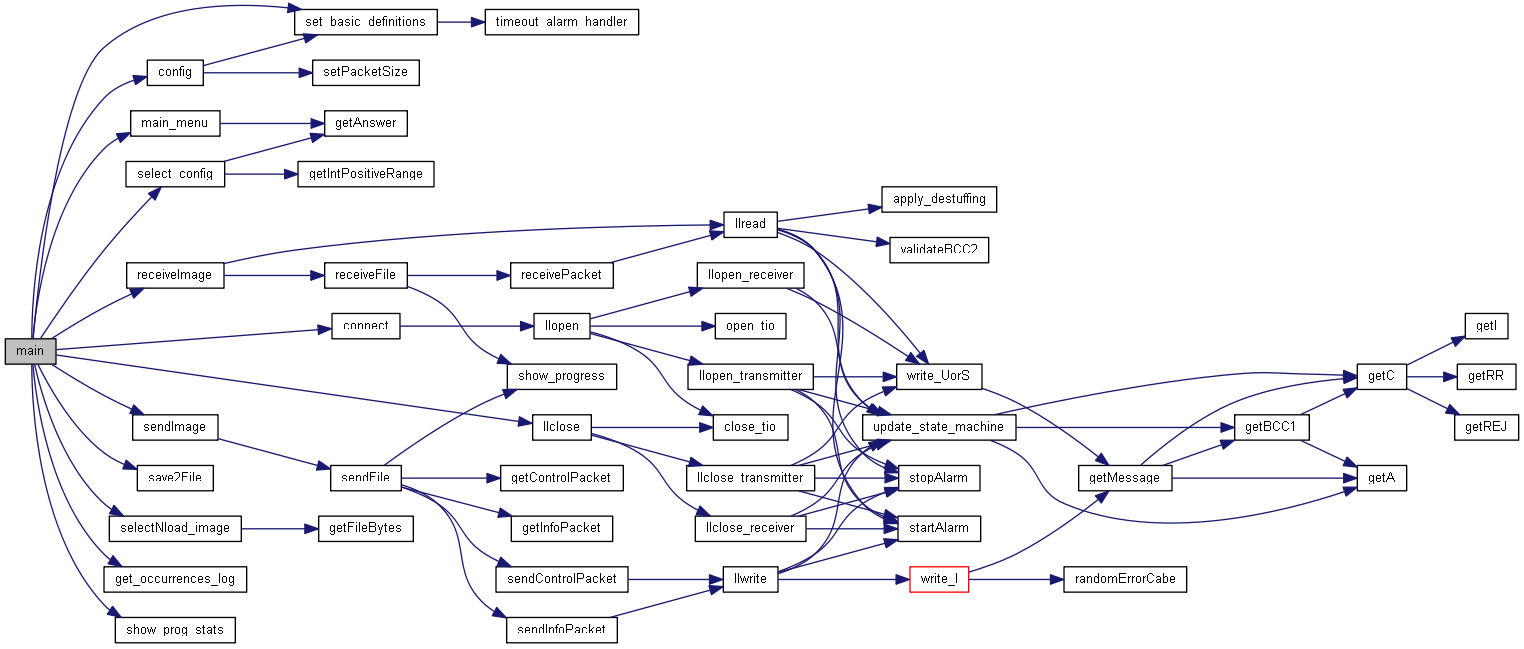
\includegraphics[width=26cm]{_app_8c_a3c04138a5bfe5d72780bb7e82a18e627_cgraph.png}
\end{sidewaysfigure}

%---------------------------------------------------------------------------------------------------------------------------------------------

\chapter{Diagrama de Módulos}
\label{modulediagram}
\centering
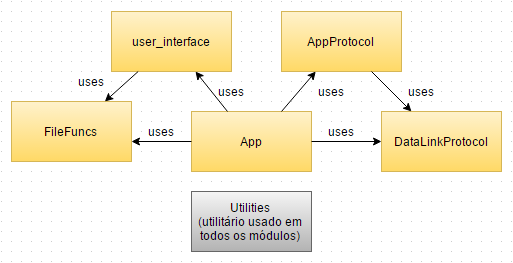
\includegraphics[width=15cm]{rcom_module_diagram.png}

\chapter{Imagens da aplicação}
\label{imagens_app}

\begin{figure}[h]
	\centering
	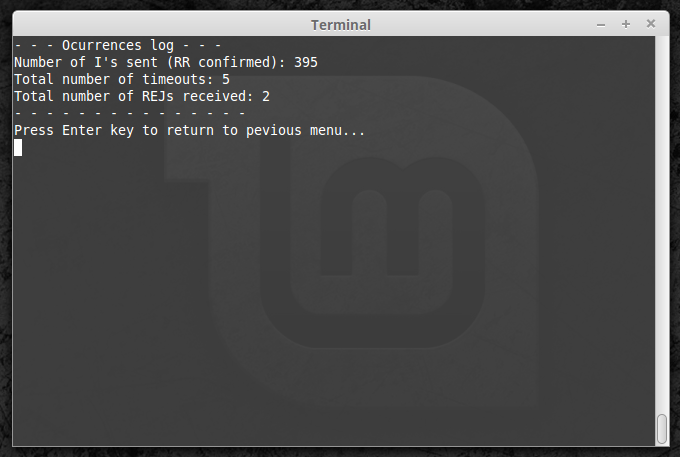
\includegraphics[width=12cm]{log.png}
	\caption{Registo de ocorrências da aplicação}
	\label{logimg}
\end{figure}

\begin{figure}[h]
	\centering
	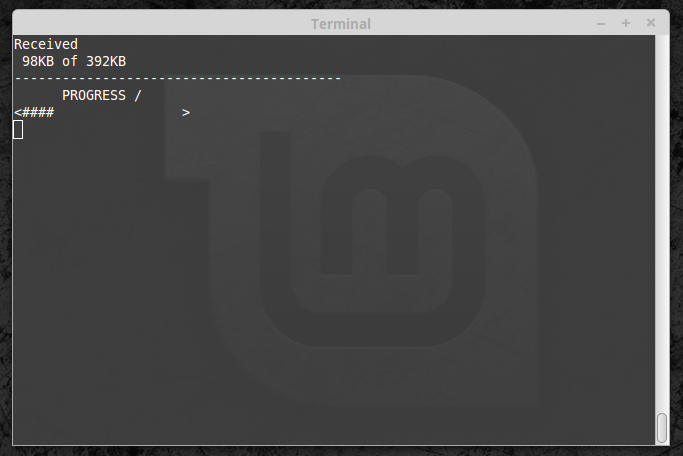
\includegraphics[width=12cm]{progress.png}
	\caption{Representação do progresso de envio/receção}
	\label{progressimg}
\end{figure}


\end{appendices}

\end{document}
